% -*- latex -*- This is a LaTeX document.
% $Id: phd-proposal.tex,v 1.2 2004-09-03 16:30:52 cananian Exp $
%%%%%%%%%%%%%%%%%%%%%%%%%%%%%%%%%%%%%%%%%%%%%%%%%%%%%%%%
\documentclass[12pt,oneside]{article}
%\usepackage{pdffonts}
\usepackage{beton}\usepackage{euler}
\usepackage{comdef}

\linespread{1.2}

\title{{\large PhD Thesis proposal for}\\
Efficient Software Transactions in Java}
\author{C. Scott Ananian}
\date{August 2004\\\vspace{5pt}}

\begin{document}
\bibliographystyle{abbrv}
\begin{titlepage}
\setlength{\baselineskip}{0.9\baselineskip}
\newcommand{\nl}{\\[0.4\baselineskip]}
\newcommand{\tight}{\\[-0.1\baselineskip]}
\newcommand{\tighter}{\\[-0.2\baselineskip]}
\begin{centering}\large
Massachusetts Institute Of Technology\tight
Department of Electrical Engineering and Computer Science\nl
%
Proposal for Thesis Research in Partial Fulfillment\tight
of the Requirements for the Degree of\tight
Doctor of Philosophy\nl
\end{centering}
\vspace{0.1cm}
\begin{tabbing}
Title: \textbf{Efficient Software Transactions in Java}\nl
Submitted By: \= C. Scott Ananian \hspace{3cm}\=\rule{6cm}{0.5pt}\tighter
              \> 29 Quincy St \#1             \>(signature)\tighter
              \> Somerville, MA 02143\nl
Date of Submission: August 2004\nl
Expected Date of Completion: December 2004\nl
Laboratory where thesis will be done: Computer Science and Artificial
Intelligence Laboratory%\nl
\end{tabbing}
Brief Statement of the Problem:

An investigation into software and hardware transaction mechanisms
is presented in the context of a sophisticated compiler for the Java
programming language.  Transactions will be presented as an organizing
principle for concurrent and fault-tolerant programming which can be
gracefully integrated with a modern object-oriented language.
Efficient software and hardware implementations of these new language
constructs will then be presented, with compiler optimizations and
microarchitectural modifications described and benchmarked.
The goal is near-zero-cost transaction implementations that will enable
``transactions-everywhere'' programming.

~\\Supervision Agreement:

The program outlined in the proposal is adequate for a doctoral
thesis.  The supplies and facilities are available, and I am willing
to supervise the research and evaluate the thesis report.

\begin{tabbing}
\hspace{3.5in}\=\kill
\>\rule{2.5in}{0.5pt}\\
\>M. Rinard, Prof. of Comp. Sci.\\
\end{tabbing}

\end{titlepage}

Although strong typing, garbage collection, and other modern
programming language constructs have enabled automatic enforcement of
many safety properties, correct concurrent and fault-tolerant
programming remains very difficult.  Programmers must keep in mind a
multitude of possible programming interleavings and fault-conditions
and mentally ensure that each candidate preserves the desired
properties of the execution.  Research on race-detection tools helps,
but a race-free program may still contain unexpected concurrent
behavior.  Language constructs such as exceptions help reason about
faults, but reconstructing a consistent view of mutated program state
after fault interrupts execution remains difficult.  What is needed is
a better mental model for reasoning about faults and concurrency

My thesis research will test the hypothesis that language-level
transactions can simplify the programmer's task by reducing the number
of alternative program states during concurrent or faulty execution.
Further, I suggest that the mechanisms for implementing
these transactions can be low-cost and easy to deploy.  I will
propose a language-level transaction model, including nesting,
recovery, and interaction with inherently non-transactional tasks like
I/O; and investigate both software and hardware mechanisms for
implementing this model.  I expect that a combined
software-hardware approach will give the best trade-off.

As part of my thesis research, I will implement transactions as part
of the FLEX research compiler for Java, which I wrote as part of my
Master's research.  I will benchmark both typical general-purpose Java
applications, as well as code specially-written to take advantage of
the transaction system, to show that it is possible to achieve good
performance.  I will also argue that transactions can significantly
reduce the time and effort required to develop concurrent and
fault-tolerant programs.

\section{Transactions}

Conventionally, atomicity in shared-memory multiprocessors is provided
via mutual-exclusion \defn{locks} (see, for example,
\cite{Tanenbaum92}[p.~35]).  Although locks are easy to
implement using test-and-set, compare-and-swap, or
load-linked/store-conditional instructions, they introduce a host of
difficulties.  To avoid deadlock when locking multiple objects, the
locks must be acquired in a consistent linear order, which makes
programming with locks error-prone and sometimes introduces
significant overheads in managing the lock acquisition protocol.
Moreover, locking can introduce other overheads, because a thread must
always grab a lock to gain exclusive access to a shared object,
regardless of whether another thread is actually attempting to access
the same object.

A transaction can be thought of as a sequence of loads and stores
performed as part of a program which either
\defn{commits} or \defn{aborts}.  If a transaction
commits, then all of the loads and stores appear to have run
atomically with respect to other transactions.  That is, the
transaction's operations are not interleaved with those of other
transactions.  If a transaction aborts, then none of its stores take
effect and the transaction may be restarted, typically using a
backoff algorithm to preclude live-lock.

Although transactions can be implemented using mutual exclusion
(locks), our algorithms will utilize non-blocking synchronization
\cite{Lamport77,Herlihy88,HerlihyLuMo03,MassalinPu91,GreenwaldCh96} to
exploit optimistic concurrency among transactions.  Non-blocking
synchronization offers a number of advantages; foremost for the
concerns of this paper is fault-tolerance.  A process which fails
while holding a lock within a critical region can prevent all other
non-failing processes from ever making progress.  It is in general not
possible to restore the locked data structures to a consistent state
after such a failure.  Non-blocking synchronization offers a graceful
solution to this trouble, as non-progress or failure of any one thread
will not affect the progress or consistency of other threads or the
system.

Implementing transactions using
non-blocking synchronization offers performance benefits as well.
Even in a failure-free system, page faults, cache misses, context
switches, I/O, and other unpredictable events may result in delays to the
entire system when mutual exclusion is used to guarantee the atomicity
of operation sequences; non-blocking
synchronization allows undelayed processes or processors to continue
to make progress.
Similarly, in real-time systems, the use of non-blocking
synchronization can prevent \emph{priority inversion} in the system
\cite{Jones97}.

The transaction model is a natural means to express both desired
atomicity and fault-tolerance properties.  In my thesis research, I will also
show how transactions can be used as a general exception-handling
mechanism and to implement back-tracking.  The transactional model can be
integrated into Java,  ``transactifying'' existing code to fix
existing concurrency bugs and using transactions for fault-tolerance,
backtracking, exception-handling, and concurrency control in new
programs.

I will explore both software and hardware implementations of this
model.  Previous implementation work has concentrated on the
\defn{Transactional memory} abstraction
\cite{Knight86,HerlihyMo93,StoneStHe93,RajwarGo02,ShavitTo95,HerlihyLuMoSc03},
which has
been proposed as a general and flexible way to allow programs to read
and modify disparate primary memory locations atomically as a single
operation, much as a database transaction can atomically modify many
records on disk.

\defn{Hardware transactional memory} (HTM) supports atomicity through
architectural means, whereas \defn{software transactional memory}
(STM) supports atomicity through languages, compilers, and libraries.
Researchers of both HTM and STM commonly express the opinion that
transactions need never touch many memory locations, and hence it is
reasonable to put a (small) bound on their size.  For HTM implementations,
they conclude that a small piece of additional hardware---typically in
the form of a fixed-size content-addressable memory and supporting
logic---should suffice.  For STM implementations, some researchers
argue additionally that transactions occur infrequently, and hence the
software overhead would be dwarfed by the other processing done by an
application.

In contrast, this thesis work will assume that transactions may be of
arbitrary size and duration, and that details of the implement should
not be exposed to the programmer of the system.  Our goal is to make
concurrent and fault-tolerant programming easier, hopefully without
incurring much 
overhead in its implementation.  I am interested in unbounded
transactions because neither programmers nor compilers can easily cope
when an architecture imposes a hard limit on transaction size.  An
implementation might be optimized for transactions below a certain
size, but must still operate correctly for larger transactions.  The
size of transactional hardware should be an implementation parameter,
like cache size or memory size, which can vary without affecting the
portability of binaries.

\subsection{Language-level Approaches to Synchronization}

Our work on integrating transactions into the Java programming
language is related to prior work on integrating synchronization
mechanisms for multiprogramming, and in particular, to prior work on
synchronization in an object-oriented framework.

The Emerald system \cite{BlackHuJuLe86,JulSt91} introduced
\emph{monitored objects} for synchronization.  Emerald code to
implement a simple directory object is shown in
Figure~\ref{fig:emerald-dir}.  Each object is associated with
Hoare-style monitor, which provides mutual exclusion and process
signalling.  Each Emerald object is divided into a monitored part and
a non-monitored part.  Variables declared in the monitored part are
shared, and access to them from methods in the non-monitored part is
prohibited---although non-monitored methods may call monitored methods
to effect the access.  Methods in the monitored part acquire the monitor lock
associated with the receiver object before entry and release it on
exit, providing for mutual exclusion and safe update of the shared
variables.  Monitored objects naturally integrate synchronization into
the object model.

Unlike Emerald monitored objects, where methods can only acquire the
monitor of their receiver and where restricted access to shared
variables is enforced by the compiler, Java implements a loose
variant where any monitor may be explicitly acquired and no shared
variable protection exists.  As a default, however, Java methods
declared with the {\tt synchronized} keyword behave like Emerald
monitored methods,
ensuring that the monitor lock of their receiver is held during execution.

Java's synchronization primitives arguably allow for more efficient
concurrent code than Emerald's---for example, Java objects can use
multiple locks to
protect disjoint sets of fields, and coarse-grain locks can be used
which protect multiple objects---but Java is also more prone to programmer
error.  However, even Emerald's restrictive
monitored objects are not sufficient to prevent data races.  As a
simple example, imagine that an object provided two monitored methods
{\tt read} and {\tt write} which accessed a shared variable.
Non-monitored code can call {\tt read}, increment the value returned,
and then call {\tt write}, creating a classic race condition scenario.
The atomicity of the parts is not sufficient to guarantee atomicity of
the whole \cite{FlanaganQa03}.

This suggests that a better model for synchronization in
object-oriented systems is \emph{atomicity}.  Figure~\ref{fig:atomic}
shows Java extended with an \atomic keyword to implement an
object representing a bank account.  Rather than explicitly
synchronizing on locks, I simply require that the methods marked
\atomic execute atomically with respect to other threads in the
system; that is, that every execution of the program computes the same
result as some execution where all atomic methods were run \emph{in
  isolation} at a certain point in time, called the
\defn{linearization point}, between their invocation and return.
Note that
atomic methods invoked directly or indirectly from an atomic
method are subsumed by it: if the outermost method appears atomic,
then by definition all inner method invocations will also appear atomic.
Flanagan and Qadeer provide a more formal semantics in \cite{FlanaganQa03}.
Atomic methods can be analyzed using sequential reasoning techniques, which
significantly simplifies reasoning about program correctness.

Atomic methods can be implemented using locks.  A simple if inefficient
implementation would simply acquire a single global lock during
the execution of every atomic method.  Flanagan and Qadeer
\cite{FlanaganQa03} present a more sophisticated technique which proves that
a given implementation using standard Java monitors correctly
guarantees method atomicity.

I will base my integration of transactions into Java on the use of
non-blocking synchronization to implement atomic methods.

\section{Example and Motivation}
I present three examples in this section, illustrating how
transactions can support fault-tolerance and back-tracking,
simplify locking, and provide a more intuitive
means for specifying thread-safety properties.
I will first examine a destructive traversal algorithm, showing how a
transaction implementation can be treated as an exception-handling
mechanism.   I then, using a network flow example, show how this
transaction mechanism can be used to simplify
the locking discipline required when synchronizing concurrent
modifications to multiple objects
Finally, I show an existing race in the Java standard libraries (in 
the class \texttt{java.lang.StringBuffer}).  ``Transactification'' of
the existing class corrects this race.

\subsecput{destruct}{Destructive traversal}
Many recursive data structures can be traversed without the use of an
stack using pointer reversal.  This technique is widely used in
garbage collectors, and was first demonstrated in this context by
Schorr and Waite \cite{SchorrWa67}.  The following code implements a
pointer-reversal traversal of a simple singly-linked list:
 \par {\footnotesize\samepage
\begin{verbatim}
// destructive list traversal.
void traverse(List l) {
  List last = null, t;
  
  /* zip through the list, reversing links */
  for (int i=0; i<2; i++) {
    do {
      if (i==0) visit(l); // visit node
      t = l.next;
      l.next = last;
      last = l;
      l = t;
    } while (l!=null);
    l = last;
    // now do again, backwards. (restoring links)
  }
}
\end{verbatim}
}
This function traverses the list, visiting nodes in order and then
reversing the {\tt next} pointer.  When the end of the list is
reached, the reversed links are traversed to restore the list's original
state.  

Of course, I've chosen the simplest possible data structure here, but
the technique works for trees and graphs---and the reader may mentally
substitute their favorite hairy update on a complicated data
structure.

In normal execution, the data structure is left complete and intact
after the operation.  But
imagine that an exception or fault occurs inside the {\tt visit()} method
at some point during the traversal: an assertion fires, an exception
occurs, the hardware hiccups, or a thread is killed.  Control may
leave the {\tt traverse()} method, but the data structure is left in
shambles.  What is needed is some exception-handling procedure to
restore the proper state of the list.  This can be manually coded with
Java's existing {\tt try}/{\tt catch} construct, but the
exception-handling code must be tightly-coupled to the traversal if it
is going to undo the list mutations.

\note{Used to have a try/catch with explicit fail in here.}
Instead, I can provide a non-deterministic choice operator,
{\tt try}/{\tt else}, and write the recovery code at a higher-level as:
\par {\footnotesize\samepage
\begin{verbatim}
try {
  traverse(list);
} else { // try-else construct
  throw new Error();
}
\end{verbatim}
}\note{I'd prefer `fail t' here, but that raises the question of how
  to export objects from transactional contexts.}

The {\tt try}/{\tt else} block appears to make a non-deterministic
choice between executing the {\tt try} or the {\tt else} clause,
depending on whether the {\tt try} would succeed or not.
I implement this with a transaction around the traversal,
always initially attempting
the {\tt try}.  Exceptions or faults cause the transaction to abort;
when it does so all the
heap side-effects of the {\tt try} block disappear.

Introducing an explicit {\tt fail} statement allows us to use the same
{\tt try}/{\tt else} for back-tracking search.

\subsecput{flow}{Network flow}

I'll turn our attention now to parallel codes.
Consider a serial program for computing network flow (see, for
example, \cite[Chapter 26]{CormenLeRi01}).  The inner loop of the code
pushes flow across an edge by increasing the ``excess flow'' on one
vertex and decreasing it by the same amount on another vertex.  One
might see the following Java code: \par {\footnotesize\samepage
\begin{verbatim}
void pushFlow(Vertex v1, Vertex v2, double flow) {
  v1.excess += flow; /* Move excess flow from v1 */
  v2.excess -= flow; /* to v2.                   */
}
\end{verbatim}
}

To parallelize this code, one must preclude multiple threads from
modifying the excess flow on those two vertices at the same time.
Locks provide one way to enforce this mutual exclusion: 
\par {\footnotesize\samepage
\begin{verbatim}
void pushFlow(Vertex v1, Vertex v2, double f) {
  Object lock1, lock2;
  if (v1.id < v2.id) {       /* Avoid deadlock. */
    lock1 = v1; lock2 = v2;
  } else {
    lock1 = v2; lock2 = v1;
  }
  synchronized(lock1) {
    synchronized(lock2) {
      v1.excess += f; /* Move excess flow from v1 */
      v2.excess -= f; /* to v2.                   */
    } /* unlock lock2 */
  } /* unlock lock1 */
}
\end{verbatim}
}

This code is surprisingly complicated and slow compared to the
original.  Space for each object's lock must be reserved.
To avoid deadlock, the code must acquire the locks in
a consistent linear order, resulting in an unpredictable branch in the
code.  In the code shown,
I have required the programmer to insert an \texttt{id} field into
each vertex object to maintain a total ordering.
The time required to acquire the locks may be
an order of magnitude larger than the time to
modify the excess flow.
\note{Using FLEX, the locking code is over 11x
  slower than the no-locks code.  With Sun's JVM, this overhead falls
  to about 1.7x, because Sun is wicked smart about their lock
  implementations.}
What's more, all of this overhead is rarely
needed!  For a graph with thousands or millions of vertices, the
number of threads operating on the graph is likely to be less than a
hundred.  Consequently, the chances are quite small that two different
threads actually conflict.  Without the locks to implement mutual
exclusion, however, the program would occasionally fail.

Software transactions (and some language support) allow the
programmer to parallelize the original code using an \texttt{atomic}
keyword to indicate that the code block should appear to execute
atomically: 
\par {\footnotesize\samepage
\begin{verbatim}
void pushFlow(Vertex v1, Vertex v2, double flow) {
  atomic { /* Transaction begin. */
    v1.excess += flow; /* Move excess flow from v1 */
    v2.excess -= flow; /* to v2.                   */
  } /* Transaction end. */
}
\end{verbatim}
} 

This {\tt atomic} region can be implemented as a transaction, and
with an appropriately non-blocking implementation, it
will scale better and execute faster than the locking version
\cite{AnanianAsKuLeLi04,HarrisFr03,GreenwaldCh96,MassalinPu91,HerlihyMo93,ShavitTo95}.
From the programmer's point of view, I've also eliminated the
convoluted locking protocol, which must
be observed rigorously everywhere the related fields are accessed if
deadlock and races are to be avoided.

Further, I can implement {\tt atomic} using the {\tt try}/{\tt else}
exception-handling mechanism I've already introduced:
 \par {\footnotesize\samepage
\begin{verbatim}
for (int b=0; ; b++) {
  try {
    // atomic actions
  } else {
    backOff(b);
    continue;
  }
  break; // success!
}
\end{verbatim}
}
\note{How hard do I try to execute the {\tt try} block?}
I non-deterministically choose to execute the body of the {\tt
  atomic} block if and only if it will be observed by all to execute
atomically.  The same linguistic mechanism I introduced for
fault-tolerance and back-tracking provides atomic regions for
synchronization as well.
\note{Mention optimistic parallelism here?}

\subsecput{stringbuffer}{The \texttt{StringBuffer} class}
The existing \defn{monitor synchronization} methodology for Java
implicitly associates an 
lock with each object.  As in Java's progenitor, Emerald
\cite{BlackHuJuLe86,JulSt91}, data races are prevented by
requiring a thread to acquire an
object's lock before touching the object's shared fields.
However, the lack of races is not sufficient to prevent unanticipated
parallel behavior.

Flanagan and Qadeer \cite{FlanaganQa03} demonstrated this
insufficiency with an
actual bug they discovered in the Sun JDK 1.4.2 Java standard
libraries.  The {\tt java.lang.StringBuffer} class,
which implements a mutable string abstraction, is implemented as follows:
\par {\footnotesize
\samepage
\begin{verbatim}
public final class StringBuffer ... {
  private char value[];
  private int count;
  ... 
  public synchronized
  StringBuffer append(StringBuffer sb) {
    ...
A:  int len = sb.length();
    int newcount = count + len; 
    if (newcount > value.length)
      expandCapacity(newcount);
    // next statement may use stale len
B:  sb.getChars(0, len, value, count);
    count = newcount;
    return this;
  }
  public synchronized int length() { return count; }
  public synchronized void getChars(...) { ... }
}
\end{verbatim}
}
The library documentation indicates that the methods of this class are meant
to execute atomically, and the {\tt synchronized} modifiers on the
methods are meant to accomplish this.

However, the {\tt append()} method is \emph{not} atomic.  Another
thread may change the length of the parameter \texttt{sb} (by adding
or removing characters) between the call to \texttt{sb.length()} at
label A and the call to \texttt{sb.getChars(\ldots)} at label B.
This non-atomicity may cause incorrect data to be appended to the
target or a \texttt{StringIndexOutOfBoundException} to be thrown. 
Although the calls to
\texttt{sb.length()} and \texttt{sb.getChars()} are individually
atomic, but they do not compose to form an atomic implementation of
\texttt{append()}.  
%The simple monitor synchronization scheme breaks
%down when operations touch multiple objects.

Note however that replacing {\tt synchronized} with {\tt atomic} in
this code gives us the semantics
we desire: the atomicity of nested {\tt atomic} blocks is guaranteed
by the atomicity of the outermost block, ensuring that the entire
operation appears atomic.

Both the network flow example and this {\tt StringBuffer} example require
synchronization of
changes to more than one object.
Monitor synchronization is not
well-suited to this task.  Atomic regions implemented with
transactions can be used to simplify the locking discipline required
to synchronize multi-object mutation
and provide a more intuitive specification for the desired
concurrent properties.  Further, the {\tt StringBuffer} example shows
that simply replacing {\tt synchronized} with {\tt atomic} provides a
alternative semantics which may in fact correct existing
synchronization errors.
For many Java programs, the
semantics of {\tt atomic} and {\tt synchronized} are identical.
\note{Can I make this rigorous?}

\subsecput{xlimit}{Limitations}
The transaction mechanism presented here is not a universal
replacement for all synchronization.  In particular, transactions
cannot replace blocking producer-consumer queues and mutual exclusion
required to serialize I/O, although the needed locks can certainly be
built with transactions.  Integrating I/O within a transactional
context remains poorly understood.  However, large programs---the
Linux kernel, for example---have been written such that locks are
never held across context switches or I/O operations.  Transactions
provide a complete solution for this limited synchronization.

\vspace*{5mm}
I have designed an implementation of software transactions which allows
us to efficiently implement the {\tt try}/{\tt else} and {\tt atomic}
constructs.  I have evaluated it by automatically
``transactifying'' Java applications by replacing synchronization with
{\tt atomic} blocks, and in \secref{properties} I present
experimental results describing the
transaction properties of programs so transformed.
I then present our software transaction design, based on the
properties I observed in our benchmarks.
\punt{
I present modelling results affirming the correctness of the design, and compiler
optimizations to enhance its performance.  I also describe a variant
on the scheme which uses some hardware support.  Finally, I present
performance data for our pure-software and partially-hardware
transaction implementations.
}

\secput{auto}{Creating transactions}
One of the difficulties of proposing a novel language feature is the
lack of benchmarks for its evaluation.  Although there is no body of
code yet using {\tt atomic} regions, there is a substantial body of
code which uses Java (locking) synchronization.  I have implemented a
compiler which substitutes {\tt atomic} blocks (methods) for {\tt
  synchronized} blocks (method) in order to evaluate the properties
Java transactions are likely to have.  Note that the semantics are not
precisely compatible: the existing Java memory model allows
unsynchronized updates to shared fields to be observed within a
synchronized block, while such updates will never be visible to an
{\tt atomic} block.  The proposed revision of the Java memory model
\cite{MansonPu02} narrows the semantic gap, however I do not treat
{\tt volatile} fields in this work.

Despite the differences in semantics, the automatic substitution of
{\tt atomic} for {\tt synchronized} does, in fact, preserve the
correctness of the benchmarks I've examined.  Moreover, as
mentioned in \secref{stringbuffer}, it
fixes the synchronization issue with {\tt java.lang.StringBuffer}.

One goal of this work was to make such improperly synchronized
applications correct and race-free, in effect fixing certain common
synchronization errors.  To this effect, I needed to preserve the
correct operation of {\tt atomic} even in the face of unsynchronized
accesses from outside the {\tt atomic} block to the fields used within
it.  Imagine unsynchronized code directly altering the length field of
{\tt StringBuffer}.  This should not cause the {\tt atomic}
{\tt StringBuffer.append()} method to appear non-atomic.
\note{Compare w/ Harris and Fraser?}

\subsecput{properties}{Properties of Transactions}
This section examines the implications of exposing the transaction
mechanism to user-level code through a compiler.
I compiled the SPECjvm98 benchmark suite with the FLEX Java compiler
\cite{Flex},
modified to turn synchronized blocks and methods into transactions,
in order to investigate the properties of the transactions in such
``automatically converted'' code.
Method splitting was performed to distinguish methods called from
within an atomic block, and nested
\texttt{atomic} blocks were implemented as a single
transaction around the outermost \texttt{atomic} region.  I
instrumented this transformed program to produce a trace of
memory references and transaction boundaries for analysis.
I found both large
transactions (touching up to 8.9 million cache lines) and frequent
transactions (up to 45 million of them).

The SPECjvm98 benchmark suite represents a variety of typical Java
applications which use the capabilities of the Java standard library.
Although the SPECjvm98 benchmarks are largely single-threaded, since
they use the thread-safe Java standard libraries they contain
synchronized code which is transformed into transactions.  Because in
this evaluation I am looking at transaction properties only, the
multithreaded \texttt{227\_mtrt} benchmark is identical to its
serialization, \texttt{205\_raytrace}.  For consistency, I present
only the latter.

\begin{figure*}
\begin{center}
\begin{tabular}{lrrrr}
        & total      &              & transactional & biggest\\
program & memory ops & transactions & memory ops    & transaction \\\hline
{\tt 201\_compress} & 2,981,777,890 & 2,272 & $<$0.1\% & 2,302 \\
{\tt 202\_jess} & 405,153,255 & 4,892,829 & 9.1\% & 7,092 \\
{\tt 205\_raytrace} & 420,005,763 & 4,177 & 1.7\% & 7,149,099 \\
{\tt 209\_db} & 848,082,597 & 45,222,742 & 23.0\% & 498,349 \\
{\tt 213\_javac} & 472,416,129 & 668 & 99.9\% & 118,041,685 \\
{\tt 222\_mpegaudio} & 2,620,818,169 & 2,991 & $<$0.1\% & 2,281 \\
{\tt 228\_jack} & 187,029,744 & 12,017,041 & 34.2\% & 14,266 \\
\end{tabular}
\end{center}
\caption{Transactification of SPECjvm98 benchmark suite: resulting
  transaction counts and sizes, compared to total number of memory
  operations (loads and stores).  These are full input size runs.
}\label{fig:perfnums}
\end{figure*}
\figput{tr-quad}{Classification of SPECjvm98 benchmarks into quadrants
based on transaction properties.}

\figref{perfnums} shows the raw sizes and frequency of transactions in
the transactified SPECjvm98 suite.
\figref{tr-quad} proposes a
taxonomy for Java applications with transactions, grouping the SPECjvm98
applications into quadrants based on the number and size of the
transactions which they perform.  Applications in Quads II and IV
require an efficient transaction implementation, because they contain
many transactional operations.
Quads III and IV contain at least some very large transactions, which
pose difficulties for currently-proposed hardware transactional memory
schemes.  I now
examine the benchmarks in each quadrant to determine why its program
logic caused it to be classified in that quadrant.

Quad I applications perform few (up to about 2000) small
transactions.  These applications include \texttt{201\_compress}, an
implementation of gzip compression, and \texttt{222\_mpegaudio}, an
MP3 decoder.  Both of these applications perform inherently serial
tasks.  They perform quite well with locks, and would likely execute
with acceptable performance even with a na\"\i{}ve software
implementation of transactions, as long as the impact on
non-transactional operations was minimal.

Quad II applications perform a large number of small transactions.
The expert system \texttt{202\_jess} falls in this category, as do
small input sizes of \texttt{209\_db}, a database.  These benchmarks
perform at least an order of magnitude more transactions than Quad
I applications, and all of the transactions are small enough to 
comfortably fit the known hardware transactional memory schemes, if
one were to be implemented.

Quad III includes \texttt{205\_raytrace}, a ray-tracing renderer.  A
small number of transactions are performed, but they may grow very
large.  Existing bounded hardware transactional schemes will not
suffice.  The large
transactions may account for a large percentage of total memory
operations, which may make software schemes impractical.

Finally, Quad IV applications such as \texttt{209\_db} and the
\texttt{213\_javac} Java compiler application perform a large number
of transactional memory operations with at least a few large transactions.  

The \texttt{213\_javac} Java compiler application and the large input
size of the \texttt{209\_db} benchmark illustrate that some programs
contain \emph{extremely} large transactions.  When \texttt{213\_javac}
is run on its full input set, it contains 4 very large transactions,
each of which contains over 118 million transactional memory
operations.  Closer
examination reveals that the method \texttt{Javac.compile()}, which
implements the entire compilation process, is marked as synchronized:
the programmer has explicitly requested that the entire compilation
occur atomically.

The \texttt{209\_db} benchmark suffers from a similar problem: at one
point the benchmark atomically scans an index vector and removes an
element, creating a potentially large transaction if the index is
large.  The size of this index is correlated in these benchmarks with
the input size, but it need not be: a large input could still result
in a small index, and (to some degree) vice-versa.

A similar situation arises in the {\tt java.lang.StringBuffer} code
shown in \secref{stringbuffer}:  a call to the synchronized
\texttt{sb.getChars()} method means that
the size of the transaction for this method will grow like the length
of the parameter~\texttt{sb}.  In other words, the transaction can be
made arbitrarily large by increasing the length of \texttt{sb}; or,
equivalently, there is no bound on transaction size without a bound on
the size of the string~\texttt{sb}.

\epsfigput{tr-sz-all}{Distribution of transaction size in the
  SPECjvm98 benchmark suite.  Note that the x-axis uses a logarithmic
  scale.}

Any scheme which allows the programmer free reign over specifying
desired transaction and/or atomicity properties will inevitably result
in some applications in each of these categories.  As existing
hardware transactional memory schemes only handle applications in Quad
I or II, they are not a good implementation technique for a general
language mechanism.  \figref{tr-sz-all} restates this problem, by
illustrating the distribution of transaction sizes in these
applications on a semi-log scale.

\punt{
\vspace*{2mm}
\begin{figure}
\begin{center}
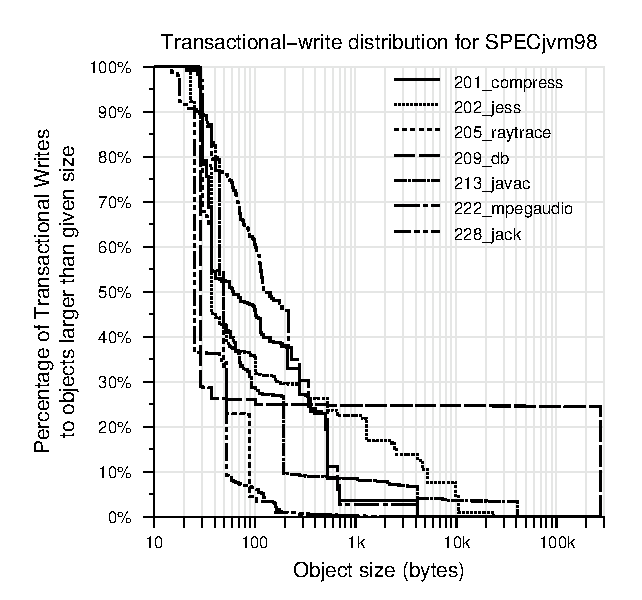
\includegraphics[width=2.25in,clip=true]{Figures/tr-w-all.eps}%
~~~~~%
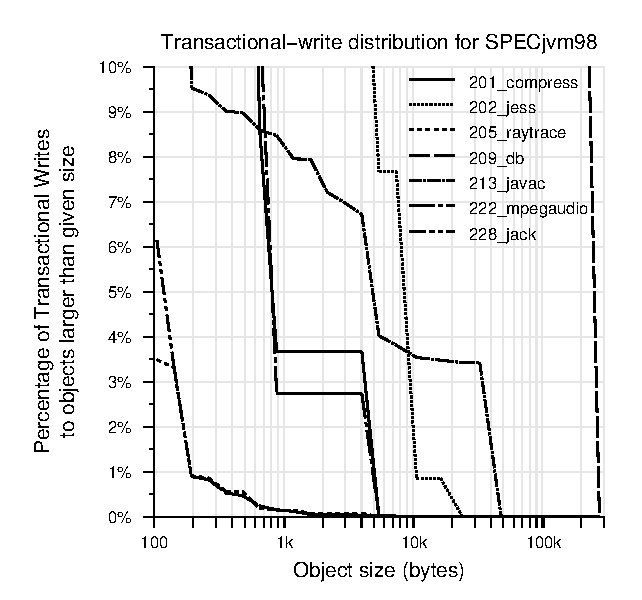
\includegraphics[width=2.25in,clip=true]{Figures/tr-w-ten.eps}%
\end{center}%
\caption{Proportion of transactional writes to objects equal to or
  smaller than a given size.  The right-hand graph zooms in on a
  portion of the relation shown in the left; note in particular that
  y-axis full-scale is only 10\% in the right-hand graph.}%
\label{fig:tr-w}%
\end{figure}%
Our software transactions implementation clones objects on
transactional writes, so that the previous state of the object can be
restored if the transaction aborts.  With this in mind, I was
interested in the number of writes to \emph{large} objects, or,
equivalently, on the object size distribution of transactional
writes.  \figref{tr-w} shows this distribution for the SPECjvm98
applications. 
}

\vspace*{5mm}

Our Java studies show that real applications can be
transactified with modest effort, yielding significant gains in
concurrency.  In other work \cite{AnanianAsKuLeLi04} we have shown
that a factor of 4 increase in concurrency can be obtained
by doing nothing more than converting locks to transactions.  Since
the transactified applications may contain large transactions,
proposed hardware support for transactions is inadequate.


\secput{efficient}{Designing Efficient Transactions}
In this section I briefly describe some desired properties of my
software transaction system.

\subsection{Field Flags}\label{sec:flagfield}
\note{Missing: performance numbers for adding check.  Use ``no trans''
version of transaction app and add check into the access functions.}
I would like non-transactional code to execute with minimal overhead,
however, transactions should still appear atomic to non-transactional
code.  Our basic mechanism is loosely based on the
distributed shared memory implementation of Scales and Gharachorloo
\cite{ScalesGh97}.  I will pick a special ``flag'' value, and
``cross-out'' locations currently involved in a transaction by
overwriting them with the flag value.  Reading or attempting to
overwrite a flagged value will indicate to non-transactional code
that exceptional processing is necessary; all other non-transactional
operations proceed as usual.

Note that our technique explicitly allows safe access to fields
involved in a transaction from non-transactional code.
\punt{
Ensuring that transactional updates remain atomic to non-transactional
code eases ``transactification'' and 
Key idea is to allow safe access by non-transactional code, so as to
allow transactification.
}

\epsfigput{bloat}{Application slowdown with increasing object bloat
for the SPECjvm98 benchmark applications.}
\subsection{Object expansion}
I will need to add some additional information to each object to
track transaction state.  I measured the slowdown caused by various
amounts of object ``bloat'' to determine reasonable bounds on the
size of this extra information.  \figref{bloat} presents these
results for the SPECjvm98 applications; I determined that two words
(eight bytes) of additional storage per object would not impact
performance unreasonably.  This amount of bloat causes a geometric
mean of 2\% slowdown on these benchmarks.

\begin{figure}
\begin{center}
\begin{tabular}{lrrrr}
        & transactional & transactional\\
program & memory ops    & stores \% \\\hline
{\tt 201\_compress} & 50,029 & 26.2\% \\
{\tt 202\_jess} & 36,701,037 & 0.6\% \\
{\tt 205\_raytrace} & 7,294,648 & 23.2\% \\
{\tt 209\_db} & 195,374,420 & 6.3\% \\
{\tt 213\_javac} & 472,134,289 & 22.9\% \\
{\tt 222\_mpegaudio} & 41,422 & 18.6\% \\
{\tt 228\_jack} & 63,912,386 & 17.0\% \\
\end{tabular}
\end{center}
\caption{Comparison of loads and stores inside transactions for the
  SPECjvm98 benchmark suite, full input runs.}
\label{fig:writepercent}
\end{figure}
\subsection{Reads vs. Writes}
\figref{writepercent} shows that transactional reads typically
outnumber transactional writes by at least 4 to 1; in some cases reads
outnumber writes by over 100 to 1.  It is worthwhile, therefore, to
make reads more efficient than writes.  In particular, since the
flag-overwrite technique discussed in \secref{flagfield} requires us
to allocate additional memory to store the ``real'' value of the
field, I wish to avoid this process for transactional reads,
reserving the extra allocation effort for transactional writes.

\punt{
\subsection{Large objects}
See \secref{properties}.
}

\secput{algo}{Software Transaction Mechanism}
I now present an algorithm which has these desired properties.
Our algorithms will be completely non-blocking, which allows good
scaling and proper fault-tolerant behavior: one faulty or slow
processor cannot hold up the remaining good processors.

I will implement the synchronization required by my algorithm using
load-linked/store-conditional instructions.  I require a particular
variant of these instructions which allows the location of the
load-linked to be different from the target of the store-conditional:
this variant is supported on the PowerPC processor family, although it
has been deprecated in the newest chips.  This disjoint location
capability is essential to allow us to keep a finger on one location
while modifying another: a poor man's ``Double Compare And Swap''
instruction.

I will describe my algorithms in the Promela modeling language
\cite{Holzmann03},
which I used to allow mechanical model checking of the race-safety
and correctness of the design.  Portions of the model have been
abbreviated for this presentation;  the full Promela model is
available from a URL given at the end of the paper.

\appref{promela} provides a brief primer on Promela syntax and semantics.

%\subsecput{interface}{Interface}
\subsecput{datastruct}{Object Structures}
\figput{tr-multi-obj}{Implementing software transactions with version
  lists.  A transaction object consists of a single field {\it
    status}, which indicates if it has COMMITTED, ABORTED, or is WAITING.
  Each object contains two extra fields: {\it readers}, a
  singly-linked list of transactions which have read this object; and
  {\it versions} a linked list of version objects.  If an object field
  is FLAG, then the value for the field is obtained from the
  appropriate linked version object.}
\figref{tr-multi-obj} illustrates the basic data structures of our
software transaction implementation.  Objects are extended with two
additional fields.  The first field, {\tt versions}, points to a
singly-linked list of object versions.  Each one contains field values
corresponding to a committed, aborted, or in-progress transaction,
identified by its {\tt owner} field.  There is a single unique
transaction object for each transaction.

The other added field, {\tt readers}, points to a singly-linked list
of transactions which have read from this object.  Committed and
aborted transactions are pruned from this list.  The {\tt readers}
field is used to ensure that a transaction does not operate with
out-of-date values if the object is later written
non-transactionally.

There is a special flag value, here denoted by {\tt FLAG}.  It should be
an uncommon value, i.e. not a small positive or negative integer
constant, nor zero.  In my implementation, I have chosen the byte
\texttt{0xCA} to be our flag value, repeated as necessary to fill out
the width of the appropriate type.
The semantic value of an object field is the value in the original
object structure, \emph{unless that value is \texttt{FLAG}}, in which
case the field's value is the value of the field in the first
committed transaction in the object's version list.  A ``false flag''
occurs when the application wishes to ``really'' store the value FLAG
in a field; this is handled by creating a fully-committed version
attached to the object and storing FLAG in that version as well as in
the object field.

\subsecput{ops}{Operations}
I support transactional read/write and non-transactional read/write
as well as transaction begin, transaction abort, and transaction
commit.  Transaction begin simply involves the creation of a new
transaction identifier object.  Transaction commit and abort are simply
compare-and-swap operations which atomically set the transaction object's {\tt
  status} field appropriately if and only if it was previously in the
WAITING state.
The simplicity of commit and abort are appealing: our algorithm
requires no complicated processing, delay, roll-back or validate
procedure to commit or abort a transaction.

I will present the other operations one-by-one.

\subsubsection{Read}

The {\tt ReadNT} function does a non-transactional read of field $f$ from
object $o$, putting the result in $v$.
In the common case, the only overhead is to check that
the read value is not FLAG.  However, if the value read \emph{is}
FLAG, we copy back the field value 
from the most-recently committed transaction (aborting all other
transactions) and try again.  The copy-back procedure will notify
us if this is a ``false flag'', in which case the value of this
field really is FLAG.  We pass the {\tt kill\_writers} constant
to the copy-back procedure to
indicate that only transactional writers need be aborted, not
transactional readers.
All possible races are confined to the copy-back procedure.
\par {\footnotesize\samepage
\begin{verbatim}
inline readNT(o, f, v) {
  do
  :: v = object[o].field[f];
     if
     :: (v!=FLAG) -> break /* done! */
     :: else
     fi;
     copyBackField(o, f, kill_writers, _st);
     if
     :: (_st==false_flag) ->
        v = FLAG;
        break
     :: else
     fi
  od
}
\end{verbatim}
}

\subsubsection{Write}
The {\tt WriteNT} function does a non-transactional write of new value $nval$
to field $f$ of object $o$.  For correctness, we need to ensure that
the reader list is empty before we do the write.  We implement this
with a load-linked/store-conditional pair, which is modelled in
Promela slightly differently, ensuring that our write only succeeds
so long as the reader list remains empty.\footnote{Note that a
  standard CAS would not suffice, as the load-linked targets a
  different location than the store-conditional.}
If it is not empty, we
call the copy-back procedure (as in {\tt readNT}), passing the
constant {\tt kill\_all} to indicate that both transactional readers
and writers should be aborted during the copy-back.  The copy-back
procedure leaves the reader list empty.

If the value to be written is actually the FLAG value, things get a
little bit trickier.  This case does not occur often, and so the
simplest correct implementation is to treat this non-transactional
write as a short transactional write, creating a new transaction for
this one write, and attempting to commit it immediately after the
write.  This is slow, but adequate for this uncommon case.
\par {\footnotesize\samepage
\begin{verbatim}
inline writeNT(o, f, nval) {
  if
  :: (nval != FLAG) ->
     do
     :: atomic {
          if /* this is a LL(readerList)/SC(field) */
          :: (object[o].readerList == NIL) ->
             object[o].fieldLock[f] = _thread_id;
             object[o].field[f] = nval;
             break /* success! */
          :: else
          fi
        }
        /* unsuccessful SC */
        copyBackField(o, f, kill_all, _st)
     od
  :: else -> /* create false flag */
     /* implement this as a short *transactional* write. */
     /* start a new transaction, write FLAG, commit the */
     /* transaction; repeat until successful. */
     /* Implementation elided. */
     ...
  fi;
}
\end{verbatim}
}
\subsubsection{Field Copy-Back}
\begin{figure}
\fontsize{6.5}{7.4}
\begin{verbatim}
inline copyBackField(o, f, mode, st) {
  _nonceV=NIL; _ver = NIL; _r = NIL; st = success;
  /* try to abort each version.  when abort fails, we've got a
   * committed version. */
  do
  :: _ver = object[o].version;
     if
     :: (_ver==NIL) ->
        st = saw_race; break /* someone's done the copyback for us */
     :: else
     fi;
      /* move owner to local var to avoid races (owner set to NIL behind
       * our back) */
     _tmp_tid=version[_ver].owner;
     tryToAbort(_tmp_tid);
     if
     :: (_tmp_tid==NIL || transid[_tmp_tid].status==committed) ->
        break /* found a committed version */
     :: else
     fi;
     /* link out an aborted version */
     assert(transid[_tmp_tid].status==aborted);
     CAS_Version(object[o].version, _ver, version[_ver].next, _);
  od;
  /* okay, link in our nonce.  this will prevent others from doing the
   * copyback. */
  if
  :: (st==success) ->
     assert (_ver!=NIL);
     allocVersion(_retval, _nonceV, aborted_tid, _ver);
     CAS_Version(object[o].version, _ver, _nonceV, _cas_stat);
     if
     :: (!_cas_stat) ->
        st = saw_race_cleanup
     :: else
     fi
  :: else
  fi;
  /* check that no one's beaten us to the copy back */
  if
  :: (st==success) ->
     if
     :: (object[o].field[f]==FLAG) ->
        _val = version[_ver].field[f];
        if
        :: (_val==FLAG) -> /* false flag... */
           st = false_flag /* ...no copy back needed */
        :: else -> /* not a false flag */
           d_step { /* LL/SC */
             if
             :: (object[o].version == _nonceV) ->
                object[o].fieldLock[f] = _thread_id;
                object[o].field[f] = _val;
             :: else /* hmm, fail.  Must retry. */
                st = saw_race_cleanup /* need to clean up nonce */
             fi
           }
        fi
     :: else /* may arrive here because of readT, which doesn't set _val=FLAG*/
        st = saw_race_cleanup /* need to clean up nonce */
     fi
  :: else /* !success */
  fi;
  /* always kill readers, whether successful or not.  This ensures that we
   * make progress if called from writeNT after a readNT sets readerList
   * non-null without changing FLAG to _val (see immediately above; st will
   * equal saw_race_cleanup in this scenario). */
  if
  :: (mode == kill_all) ->
     do /* kill all readers */
     :: moveReaderList(_r, object[o].readerList);
        if
        :: (_r==NIL) -> break
        :: else
        fi;
        tryToAbort(readerlist[_r].transid);
        /* link out this reader */
        CAS_Reader(object[o].readerList, _r, readerlist[_r].next, _);
     od;
  :: else /* no more killing needed. */
  fi;
  /* done */
}
\end{verbatim}
\caption{The field copy-back routine.}\label{fig:copyback}
\end{figure}
\figref{copyback} presents the field copy-back routine.  We create a
new version owned by a pre-aborted transaction which serves as a
reservation on the head of the version list.  We then write to the
object field with a load-linked/store-conditional pair if and only if
our version is still at the head of the versions list.\footnote{Note
  again that a CAS does not suffice.}  This addresses
the major race possible in this routine.

\subsubsection{Transactional Read}
A transactional read is split into two parts.  Before the read, we
must ensure that our transaction is on the reader list for the
object.  This is straight-forward to do in a non-blocking manner as
long as we always add ourselves to the head of the list.  We must also
walk the versions list, and abort any uncommitted transaction other
than our own.  These steps can be combined and hoisted so that they
are done once before the first read from an object and not repeated.

At read time, we initially read from the original object.  If the
value read is not FLAG, we use it.  Otherwise, we look up the version
object associated with our transaction (this will typically be at the
head of the version list) and read the appropriate value from that
version.  Note that the initial read-and-check can be omitted if we
know that we have already written to this field inside this transaction.
\par {\footnotesize\samepage
\begin{verbatim}
inline readT(tid, o, f, ver, result) {
  do
  ::
     /* we should always either be on the readerlist or
      * aborted here */
     result = object[o].field[f];
     if
     :: (result==FLAG) ->
        if
        :: (ver!=NIL) ->
           result = version[ver].field[f];
           break /* done! */
        :: else ->
           findVersion(tid, o, ver);
           if
           :: (ver==NIL) ->/*use val from committed vers.*/
              assert (_r!=NIL);
              result = version[_r].field[f];/*false flag?*/
              moveVersion(_r, NIL);
              break /* done */
           :: else /* try, try, again */
           fi
        fi
     :: else -> break /* done! */
     fi
  od
}
\end{verbatim}
}

\begin{figure}
\fontsize{6.5}{8}
\begin{verbatim}
/* per-object, before write. */
inline ensureWriter(tid, o, ver) {
  assert(tid!=NIL);
  ver = NIL; _r = NIL; _rr = NIL;
  do
  :: assert (ver==NIL);
     findVersion(tid, o, ver);
     if
     :: (ver!=NIL) -> break /* found a writable version for us */
     :: (ver==NIL && _r==NIL) ->
        /* create and link a fully-committed root version, then
         * use this as our base. */
        allocVersion(_retval, _r, NIL, NIL);
        CAS_Version(object[o].version, NIL, _r, _cas_stat)
     :: else ->
        _cas_stat = true
     fi;
     if
     :: (_cas_stat) ->
        /* so far, so good. */
        assert (_r!=NIL);
        assert (version[_r].owner==NIL ||
                transid[version[_r].owner].status==committed);
        /* okay, make new version for this transaction. */
        assert (ver==NIL);
        allocVersion(_retval, ver, tid, _r);
        /* want copy of committed version _r.  No race because
         * we never write to a committed versions. */
        version[ver].field[0] = version[_r].field[0];
        version[ver].field[1] = version[_r].field[1];
        assert(NUM_FIELDS==2); /* else ought to initialize more fields */
        CAS_Version(object[o].version, _r, ver, _cas_stat);
        moveVersion(_r, NIL); /* free _r */
        if
        :: (_cas_stat) ->
           /* kill all readers (except ourself) */
           /* note that all changes have to be made from the front of the
            * list, so we unlink ourself and then re-add us. */
           do
           :: moveReaderList(_r, object[o].readerList);
              if
              :: (_r==NIL) -> break
              :: (_r!=NIL && readerlist[_r].transid!=tid)->
                 tryToAbort(readerlist[_r].transid)
              :: else
              fi;
              /* link out this reader */
              CAS_Reader(object[o].readerList, _r, readerlist[_r].next, _)
           od;
           /* okay, all pre-existing readers dead & gone. */
           assert(_r==NIL);
           /* link us back in. */
           ensureReaderList(tid, o);
           break
        :: else
        fi;
        /* try again */
     :: else
     fi;
     /* try again from the top */
     moveVersion(ver, NIL)
  od;
  /* done! */
  assert (_r==NIL);
}
\end{verbatim}
\caption{The per-object version-setup routine for transactional writes.}
\label{fig:ensurewriter}
\end{figure}
\begin{figure}
\fontsize{6.5}{8}
\begin{verbatim}
/* per-field, before write. */
inline checkWriteField(o, f) {
  _r = NIL; _rr = NIL;
  do
  ::
     /* set write flag, if not already set */
     _val = object[o].field[f];
     if
     :: (_val==FLAG) ->
        break; /* done! */
     :: else
     fi;
     /* okay, need to set write flag. */
     moveVersion(_rr, object[o].version);
     moveVersion(_r, _rr);
     assert (_r!=NIL);
     do
     :: (_r==NIL) -> break /* done */
     :: else ->
        object[o].fieldLock[f] = _thread_id;
        if
        /* this next check ensures that concurrent copythroughs don't stomp
         * on each other's versions, because the field will become FLAG
         * before any other version will be written. */
        :: (object[o].field[f]==_val) ->
           if
           :: (object[o].version==_rr) ->
              atomic {
                if
                :: (object[o].fieldLock[f]==_thread_id) ->
                   version[_r].field[f] = _val;
                :: else -> break /* abort */
                fi
              }
           :: else -> break /* abort */
           fi
        :: else -> break /* abort */
        fi;
        moveVersion(_r, version[_r].next) /* on to next */
     od;
     if
     :: (_r==NIL) ->
        /* field has been successfully copied to all versions */
        atomic {
          if
          :: (object[o].version==_rr) ->
             assert(object[o].field[f]==_val ||
                    /* we can race with another copythrough and that's okay;
                     * the locking strategy above ensures that we're all
                     * writing the same values to all the versions and not
                     * overwriting anything. */
                    object[o].field[f]==FLAG);
             object[o].fieldLock[f]=_thread_id;
             object[o].field[f] = FLAG;
             break; /* success!  done! */
          :: else
          fi
        }
     :: else
     fi
     /* retry */
  od;
  /* clean up */
  moveVersion(_r, NIL);
  moveVersion(_rr, NIL);
}
\end{verbatim}
\caption{The per-field copy-through routine for transactional writes.}
\label{fig:copythrough}
\end{figure}
\subsubsection{Transactional Write}
Again, writes are split in two.  Once for each object we must traverse
the version list, aborting other versions and locating or creating a
version corresponding to our transaction.  We must also traverse the
reader list, aborting all transactions on the list except ourself.
This is shown in the {\tt ensureWriter} routine in \figref{ensurewriter}.

Once for each field we intend to write, we must perform a
copy-through: copy the object's field value into all the versions and
then write FLAG to the object's field.  We use
load-linked/store-conditional to update versions only if the object's
field has not already been set to FLAG behind our backs by another
copy-through.  The {\tt checkWriteField} routine is shown in
\figref{copythrough}.

Then, for each write, we simply write to the identified version.
\par {\footnotesize\samepage
\begin{verbatim}
inline writeT(ver, f, nval) {
  /* easy enough: */
  version[ver].field[f] = nval;
}
\end{verbatim}
}

\secput{verification}{Verification}
The Promela model of this software transaction system was model
checked with Spin version 4.1.0 and verified to operate correctly and
without races.  The verification was done on an SGI 64-processor MIPS
machine with 16G of memory.

Sequences of transactional and non-transactional load and store
operations were checked using two concurrent processes, and all possible
interleavings were found to produce correct results consistent with
the semantic atomicity of the transactions.  A number of subtle race
conditions were discovered and corrected during this process.
In particular, early versions of the algorithms sometimes allowed
readers to escape being aborted while racing a writer in
createVersion, and could allow inconsistent reads.

Spin is not particularly suited to checking models with dynamic
allocation and deallocation.  In particular, it considers the
location of objects part of the state space, and allocating object
A before object B produces a different state than if object B
were allocated first.  This artificially enlarges the
state space.  A great deal of effort was expended tweaking the
model to approach a canonical allocation ordering.  A better solution
to this problem would allow larger model instances to be checked.

\punt{
\secput{eval}{Evaluation}

\begin{figure*}
\footnotesize
\begin{center}
\begin{tabular}{lr|rr|rr}
Benchmark                 &  Base       & Locks         & Trans              & Time                     & Overflow       \\
                          &             & time          & time               & in trans              & overhead       \\
                          &  (cycles)   & \multicolumn{2}{c|}{(\% of Base)}   & \multicolumn{2}{c}{(\% of Trans time)}                 \\ \hline
\texttt{200\_check}       &   8,062,716 & 124.0\%       &  101.7\%           & 32.9\%           & 0.00366\%      \\
\texttt{202\_jess}        &  75,012,964 & 140.9\%       &  107.1\%           & 59.3\%           & 0.00761\%      \\
\texttt{209\_db}          &  11,784,220 & 142.4\%       &  105.1\%           & 53.9\%           & 0              \\
\texttt{213\_javac}       &  30,688,574 & 169.9\%       & 1469.5\%           & 99.0\%           & 93.0\%         \\
\texttt{222\_mpegaudio}&  98,961,244    & 100.3\%       &   99.6\%           & 0.817\%          & 0              \\
\texttt{228\_jack}        & 261,441,564 & 175.3\%       &  104.4\%           & 32.2\%           & 0.00260\%      \\
\end{tabular}
\end{center}
\caption{SPECjvm98 performance and overheads on a 1-processor UVSIM simulation. The {\em Base }
 time uses no synchronization.  The {\em Locks time} is the time using
 locks as a percentage of the base.  The {\em Trans time} is the time using BTM
 transactions as a percentage of the base. The
 {\em time in Trans} is the fraction of the {\em Trans time} actually
 spent running a transaction.  The {\em
 Overflow overhead} column is fraction of the {\em Trans time}
 spent handling overflows.}
\label{fig:specperf}
\end{figure*}
}
\punt{
We found that using BTM transactions in the SPECjvm98 benchmarks
results in very little overhead compared to using locks. We compiled
the benchmarks to use BTM transactions using our modified Java
compiler.  The \texttt{201\_compress} and \texttt{205\_raytrace}
benchmarks were omitted due to unresolved bugs in the base UVSIM
simulator, and similarly \texttt{libpthread} deficiencies prevented
the execution of \texttt{227\_mtrt}.
The remaining benchmarks were run on one processor in UVSIM to compare the
performance overheads associated with BTM transactions compared to
locks.  As shown in \figref{specperf}, there is a significant amount
of overhead associated with locking (more than 75\% over the base case
in {\texttt{228\_jack})}. %Put that {} around the texttt to prevent the jack from being separated from the )
For BTM, there are two main sources of
overhead: The transactions may abort, wasting the cycles spent
computing, and also executing the branch to the abort handler.  For
these Java programs, the transactions never abort because they are
single-threaded programs.  The second overhead is the cost of handling
overflows.

The only application that has a significant transaction overhead is
\texttt{javac}, which runs 14 times slower under BTM than without any
mutual exclusion.  Virtually all of the overhead comes from handling
overflows, which is not surprising since the entire compilation is
enclosed in one large transaction.  The transaction touches 253,547
cache lines, and there are only 16K cache lines in the L2 cache,
meaning that the overflow memory contains at least 237K cache lines.
So even though only 0.5\% of the xops miss, those few misses incur
huge search costs, as the finite state machine looks through the
linear array of overflowed cache lines.  We intend to look into using
a better data structure, such as a hash table.  Though there is a
significant performance decrease in this case, BTM still ensures the
application runs correctly. Namely, the programmer wanted the entire
compile process to occur as one atomic action so BTM will ensure that
is the case.  It may be the case that \texttt{javac} really cannot be
parallelized, in which case locks may be the best choice.  But if the
programmer wishes to parallelize \texttt{javac}, she may be find it
easier to break up the large transaction than to break up a locked
block.
}
\secput{related}{Related work}
A number of researchers have been investigating transactional memory
systems.  This is the first paper to present a model-checked non-blocking
object-oriented system which allows co-existence of non-transactional and
transactional accesses to a dynamic set of object fields.

\subsecput{nb-sync}{Non-blocking synchronization}

Lamport presented the first alternative to synchronization via mutual
exclusion in \cite{Lamport77}, for a limited situation involving a single
writer and multiple readers.  Lamport's technique relies on reading
guard elements in an order opposite to that in which they are written,
guaranteeing that a consistent data snapshot can be recognized.  The
writer always completes its part of the algorithm in a constant number
of steps; readers are guaranteed to complete only in the absence of
concurrent writes.

Herlihy formalized \emph{wait-free} implementations of
concurrent data objects in \cite{Herlihy88}.  A wait-free implementation
guarantees that any process can complete any operation in a finite
number of steps, regardless of the activities of other processes.
Lamport's algorithm is not wait-free
because readers can be delayed indefinitely.

Massalin and Pu introduced the term \emph{lock-free} to describe 
algorithms with weaker progress guarantees.
A lock-free implementation guarantees only that \emph{some}
process will complete in a finite number of steps
\cite{MassalinPu91}.  Unlike a wait-free implementation,
lock-freedom allows starvation.  Since other simple techniques can be
layered to prevent starvation (for example, exponential backoff),
simple lock-free implementations are usually seen as worthwhile practical
alternatives to more complex wait-free implementations.

An even weaker criterion, \emph{obstruction-freedom}, was introduced
by Herlihy, Luchangco, and Moir in \cite{HerlihyLuMo03}.
Obstruction-freedom only guarantees progress for threads executing in
isolation; that is, although other threads may have partially
completed operations, no other thread may take a step until the
isolated thread completes.  Obstruction-freedom not only allows
starvation of a particular thread, it allows contention among threads
to halt all progress in all threads
indefinitely.  External mechanisms are used to reduce contention
(thus, achieve progress) including backoff, queueing, or timestamping.

We will use the term \emph{non-blocking} to describe
generally any synchronization mechanism which doesn't rely on mutual
exclusion or locking, including wait-free, lock-free,
and obstruction-free implementations.
We will be concerned mainly with lock-free algorithms.%
\footnote{Note that some authors use ``non-blocking'' and
  ``lock-free'' as synonyms, usually meaning what we here call
  \emph{lock-free}.  Others exchange our definitions for ``lock-free''
  and ``non-blocking'', using lock-free as a generic term and non-blocking
  to describe a specific class of implementations.  As there is
  variation in the field, we choose to use the parallel construction
  \emph{wait-free}, \emph{lock-free}, and \emph{obstruction-free} for
  our three specific progress criteria, and the dissimilar
  \emph{non-blocking} for the general class.}

\subsecput{efficiency}{Efficiency}
Herlihy presented the first \emph{universal} method for wait-free
concurrent implementation of an arbitrary sequential object
\cite{Herlihy88,Herlihy91}.  This original method was based on
a \emph{fetch-and-cons} primitive, which atomically places
an item on the head of a list and returns the list of items following
it; all concurrent primitives capable of solving the
$n$-process consensus problem---\emph{universal} primitives---were
shown powerful enough to implement \emph{fetch-and-cons}.
In Herlihy's method, 
every sequential operation is translated into two steps.  In the first,
\emph{fetch-and-cons} is used to place the name and arguments of the
operation to be performed
at the head of a list, returning the other operations on the list.
Since the state
of a deterministic object is completely determined by the history of
operations performed on it, applying the operations returned
in order from last to first is sufficient to locally reconstruct the
object state 
prior to our operation.
We then use the prior state to compute the result of our operation
without requiring further synchronization with the other processes.

This first universal method was not very practical, a shortcoming
which Herlihy soon addressed \cite{Herlihy93}.  In addition, his revised universal
method can be made lock-free, rather than wait-free, resulting in
improved performance.  In the lock-free version of this method,
objects contain a shared variable
holding a pointer to their current state.  Processes begin by loading
the current state pointer and then copying the referenced state to a
local copy.  The sequential operation is performed on the
copy, and then if the object's shared state pointer is unchanged from
its initial load it is atomically swung to point at the updated state.

Herlihy called this the ``small object protocol'' because the object
copying overhead is prohibitive unless the object is small enough to
be copied efficiently (in, say, $O(1)$ time).  He also presented a
``large object protocol'' which requires the programmer to
manually break the object into small blocks, after which the small
object protocol can be employed. 
\punt{ This trouble with large objects is
common to many non-blocking implementations; our solution is presented
in \secref{proposal}.}

Barnes provided the first universal non-blocking implementation
method which avoids object copying \cite{Barnes93}.  He eliminates the
need to store ``old'' object
state in case of operation failure by having all threads cooperate to
apply operations.  For example, if the first processor begins an operation
and then halts, another processor will complete the operation of the first
before applying its own.  Barnes proposes to accomplish the
cooperation by creating a parallel state machine for each operation,
so that each thread can independently try to advance the machine from state
to state and thus advance incomplete operations.%
\footnote{It is interesting to note that Barnes' cooperative method
  for non-blocking 
  situation plays out in a real-time system very similarly to priority
  inheritance for locking synchronization.}
Although this avoids
copying state, the lock-step cooperative process is extremely
cumbersome and does not appear to have ever been implemented.
Furthermore, it does not protect against errors in the implementation
of the operations, which could cause \emph{every} thread to fail in turn
as one by one they attempt to execute a buggy operation.

Alemany and Felten \cite{AlemanyFe92} identified two factors hindering the
performance of non-blocking algorithms to date: resources wasted by operations
that fail, and the cost of data copying.  Unfortunately, they
proceeded to
``solve'' these problems by ignoring short delays and failures and
using operating system support to handle delays caused by
context switches, page faults, and
I/O operations.  This works in some situations, but obviously suffers
from a bootstrapping problem as the means to implement an operation system.

Although lock-free implementations are usually assumed to be more
efficient that wait-free implementations, LaMarca \cite{LaMarca94}
showed experimental evidence that Herlihy's simple
wait-free protocol scales very well on parallel machines.
When more than about twenty threads are involved, the wait-free
protocol becomes
faster than Herlihy's lock-free small-object protocol, three OS-aided
protocols of LaMarca and Alemany and Felten, and a
\emph{test-and-Compare\&Swap} spin-lock.

% Afek et al have a somewhat complicated improved wait-free method.

% Transactional memories?
\subsecput{tm}{Transactional Memory Systems}

Several software transaction systems have been proposed.  Some constrain the
programmer and make transactions difficult to use.  All have
relatively high overheads, which make transactions unattractive for
uniprocessor and small SMP systems. [Once the number of processors is
large enough, the increased parallelism which can be provided by
optimistic transactions may cancel out the performance penalty of
their use.]

The first proposal for software transactional memory was proposed by
Shavit and Touitou \cite{ShavitTo95}; their system requires that all
input and output locations touched by a transaction be known in
advance, which limits its application.  It performs at least 10
fetches and 4 stores per location accessed (not counting the loads and
stores directly required by the computation).  The benchmarks
presented were run on between 10 and 64 processors.

Rudys and Wallach \cite{RudysWa02} proposed a copying-based
transaction system to allow rollback of hostile codelets.
They show an order of magnitude slowdown for field and array
accesses, and 6x to 23x slowdown on their benchmarks.

Herlihy, Luchango, Moss, and Scherer's scheme \cite{HerlihyLuMoSc03}
allows transactions to touch a dynamic set of memory locations;
however the user still has to explicitly \emph{open} every object touched
before it can be used in a transaction.  This implementation is based
on object copying, and so has poor performance for large objects and
arrays.  Not including work necessary to copy objects involved in
writes, they require $O(R(R+W))$ work to open $R$ objects for reading
and $W$ objects for writing, which may be quadratic in the number of objects
involved in the transaction.   A list insertion benchmark which they
present shows 9x slowdown over a locking scheme, they beat the locking
implementation when more than 5-10 processors are active.  They
present benchmark data with up to 576 threads on 72 processors.

Harris and Fraser built a software transaction system on a flat
word-oriented transactional memory abstraction \cite{HarrisFr03},
roughly similar to simulating Herlihy's original hardware
transactional memory proposal in software.  This avoids problems with
large objects.  Performing $m$ memory operations touching $l$ distinct
locations costs at least $m+l$ extra reads and $l+1$ CAS operations, in
addition to the reads and writes required by the computation.
They appear to execute about twice as slowly as a locking
implementation on some microbenchmarks.  They benchmark on a
4-processor as well as a 106-processor machine; their crossover point
(at which the blocking overhead of locks matches the software
transaction overhead) is around 4 processors.
Note that Harris and Fraser do not address the problem of
concurrent non-transactional operations on locations involved in a
transaction.  Java synchronization allows such concurrent operations,
with semantics given by the Java memory model \cite{MansonPu02}.
We support these operations safely using our FLAG mechanism.

Programmers will be reluctant to use transactions to synchronize their
code when it results in their code running more slowly on the uniprocessor
and small-SMP systems which are most common today.
\note{Segue into hardware transactions writeup?}

Our SPECjvm98 and Linux case studies indicate that
transactional memory operations can be extremely common when
transactions are made easy to use and natural to express.  Programmers
can be expected to use both very small and very large transactions
when they are able, and transactions are used by the operating system
and programming libraries to provide synchronization and safety
properties.  Implementing transactional memory in hardware allows the
overheads to be low\note{\textbf{cite figures here}}, which is appropriate
when transactional operations are common.

%%%%%%%%%%%%%%%%%%%%%%%%%%%%%%%
\punt{
Ideas:
 - virtual memory/overlays comparison
 - what is expensive in software versions XBEGIN?  XLD?
 - basic ideas of software impls
   also, how they handle overflow & other limits.
 - honest about what we're showing.
   here's what happens if you explore the hardware avenue.
   sw technology problems become solved hw problems.
 - k-compare-and-swap insufficient?
 - say when we couldn't find performance numbers.
   performance #s in terms of reads/writes.
 - now that we know what transactions look like,
   we want to use BTM\@.
 - use categories?
 - STM systems always use ridiculously large # processors for benchmarks.

The software just ain't good enough!
\begin{itemize}
\item Argue that SW isn't good
\item Also, lots of transactional loads and stores
\end{itemize}

Software transactional memory implementations:
% FOR EACH: PERFORMANCE.  IDEA.  LIMITS.
\begin{itemize}
\item Shavit and Touitou \cite{ShavitTo95}: static transactions only;
  that is, input and output locations must be known in advance.
  Performance?
  Non-blocking, based on LL/SC. k-word compare\&swap operation.
  ``outperforms Herlihy's translation method for sufficiently large
  numbers of processors.''  Alleges Herlihy/Moss is blocking?
  I think this is actually the case.  Our scheme is not.
  Elsewhere, ``but not non-blocking, since a single process which is
  repeatedly swapped during the execution of a transaction will never
  terminate successfully''.  They define non-blocking as ``repeated
  execution of some transaction by a process implies that some process
  (not necessarily the same one and with a possibly different
  transaction) will terminate successfully after a finite number of
  attempts in the whole system.''
  ``static transactions, that is, transactions which access a
  pre-determined sequence of locations.  This class includes most of
  the known and proposed synchronization primitives in the
  literature.''
  Requires one ownership record for every location in the memory.
  no limits to size of trans, since we allocate one ownership record
  per memory location.

  Performance: *at least* 5 fetches, 5 LL, and 4SC per location
  accessed.

  64 processors; no numbers presented for less than 10 processors.

  acquire/release/agree are expensive.

\item Rudys and Wallach \cite{RudysWa02}: transactions for security.
  6x to 23x slowdown.  Creates 'backup' objects.  Predictably bad
  for large objects.  10x slowdown for field/array accesses.
  only uniprocessor.

\item Herlihy et al \cite{HerlihyLuMoSc03}: dynamic transactions, but
  copies entire object and so works for small objects only.  Basically
  Herlihy's method.  You must explicitly \emph{open} every object
  accessed, at which time conflict-checking is done.
  O((R+W)R) work to open R objects for reading and W objects for
  writing, plus cost to copy W objects once.  Concretely: for simple
  list insert/delete, locks perform 768 ops/ms, and best DSTM scheme
  is 80 ops/ms.   So over 9x slowdown.
  Up to 576 threads on 72 processors.

  open and commit are the expensive operations.
\item Harris and Fraser \cite{HarrisFr03}: atomic sections, word-based
  scheme.  no safety for non-transactional operations which might
  touch transactional locations.  transactional operation at least 2x
  slower than normal op.
  XBEGIN = CAS + STORE
  XFAIL = STORE
  Tread = 2 FETCH (best case)
  Twrite = 1 FETCH + (1 FETCH and 2 STOREs, on same cache line)
  XEND = > (1 FETCH + 1 CAS) for each distinct word read or written.

  overhead of a committing transaction performing r reads and w writes
  to 'l' distinct locations.
  is at least (2r+2w+(l)) reads (2w+1) writes, and (l+1) CAS
  operations.  2(r+w)+l reads, 2w+1 writes, and (l+1) CAS operations.

m memory operations to l locations does m+l extra reads and l+1 CAS operations.

  4 proc; also 48 proc of 106-processor machine.  I think the
  crossover point is around 4 proc.

  COMMIT is the most expensive operation.
\end{itemize}
}


\section{Expected Contributions}

\subsecput{contrib}{Contributions}
The contributions of this thesis include:
\begin{itemize}
\item A way to ``transactify'' existing Java programs, and a
  description of the transaction properties of typical Java programs
  transformed in such a way.
\item A concrete language design to integrate transactions into Java
  providing fault-tolerance, backtracking, and non-blocking
  synchronization.
%\note{This is \texttt{try \{\ldots\} else \{\ldots\}} syntax.}
%\note{Omitting ``optimistic concurrency'' from this list for now.}
\item An efficient implementation of this design which extends
  race-protection to unsynchronized code.
\item A mechanically-verified Promela model of the implementation.
\item Empirical data to justify the design choices.
\punt{
\item Compiler optimizations to improve the speed of software
  transactions.
\item An application of fast functional arrays to solve the ``large
  object'' problem with Herlihy's universal non-blocking protocol.
  \note{Short section; cite my Area Exam as a Technical Report here
  for more details. Omit this?}
\item A variation of the implementation which leverages hardware
  support for small transactions.  This allows hardware small
  transactions to be bootstrapped to provide efficient large
  transactions.
}
\end{itemize}

We have outlined a mechanism to integrate transactions into an object
oriented language to provide fault-tolerance, back-tracking, and
non-blocking synchronization.  We have also shown the potential for
automatically ``transactifying'' existing Java programs, and presented
empirical data on the properties of these transactified applications.
We have
presented an efficient implementation of software transactions which
has been verified with the Spin model checker to be correct and race
free.

\section*{Acknowledgments}
Charles E. Leiserson suggested the ``network flow'' example in
\secref{flow}.
\punt{Sean Lie adapted the hardware simulator which
provided the timings in \figref{hw-timings}.}

\section*{Spin model for Software Transactions}
The complete Spin 4.1.0 model for the FLEX software transaction system is
available for download at
\url{http://flex-master.csail.mit.edu/Harpoon/swx.pml}.

%\renewcommand{\baselinestretch}{1}
\bibliographystyle{plain}
\bibliography{xaction}

\clearpage
\appendix
\secput{promela}{Promela Primer}
A concise Promela reference is available at
\url{http://spinroot.com/spin/Man/Quick.html}; we will here attempt to
summarize just enough of the language to allow the model we've
presented in this paper to be understood.

Promela syntax is C-like, with the same lexical and commenting
conventions.  Statements are separated by either a semi-colon, or,
equivalently, an arrow.  The arrow is typically used to separate a
guard expression from the statements it is guarding.

The program counter moves past a statement only if the statement is
{\it enabled}.  Most
statements, including assignments, are always enabled.
A statement consisting only of an expression is enabled iff the
expression is true (non-zero).
Our model uses three basic Promela statements: selection, repetition,
and {\tt atomic}.

The selection statement,
%\par{\footnotesize\samepage
\begin{verbatim}
if
:: guard -> statements
...
:: guard -> statements
fi
\end{verbatim}
%}
selects one among its options and executes it.  An option can be
selected iff its first statement (the guard) is enabled.  The
special guard {\tt else} is enabled iff all other guards are not.

The repetition statement,
%\par{\footnotesize\samepage
\begin{verbatim}
do
:: statements
...
:: statements
fi
\end{verbatim}
%}
is similar: one among its enabled statements is selected and executed,
and then the process is repeated (with a different statement possibly
being selected each time) until control is explicitly transfered out
of the loop with a {\tt break} or {\tt goto}.

Finally,
%\par{\footnotesize\samepage
\begin{verbatim}
atomic { statements }
\end{verbatim}
%}
executes the given statements in one indivisible step.  For the
purposes of this model, a {\tt d\_step} block is functionally identical.
Outside {\tt atomic} or {\tt d\_step} blocks, Promela allows
interleaving before and after every statement, but statements are
indivisible.

Functions as specified in this model are similar to C macros: every
parameter is potentially both an input {\it and} an output.  Calls to
functions with names starting with {\tt move} are simple assignments;
they've been turned into macros so that reference counting
can be performed.

\punt{
\secput{extra}{Text with nowhere else to go}

\begin{figure*}
\footnotesize
\begin{center}
\begin{tabular}{l@{}rrrrrrrrr}
program  & input& total      & \% cache  & xactions    & oversized & xops        & xmiss & overflow & biggest \\ 
         & size & memory ops & misses &             & xactions  &   \%        &   \%    & \% & xaction\\ \hline
\texttt{make\_linux}  &  & 315,776,028 & 0.56\%  &  6,964,277  & 3368     & 41.0\%  &  0.017\%  &            &         8144   \\
\texttt{dbench}      &  & 100,928,220 & 0.43\%  &  1,863,426  &   88     & 49.5\%  &  0.001\%  &            &         7047   \\

 \hline \texttt{201\_compress } &   1 & 229,332,212 &  0.10\% &        524 &   0 &  0.0\% &     0   &      0   &     1,335 \\
                                &  10 & 264,389,092 &  0.10\% &        662 &   0 &  0.0\% &     0   &      0   &     1,335 \\
                               & 100 & 2,981,777,890 &  0.10\% &      2,272 &   0 &  0.0\% &     0   &      0   &     1,352 \\
 \hline \texttt{202\_jess     } &   1 &   1,972,479 &  3.13\% &     82,103 &   0 & 43.3\% &     0   &      0   &     3,586 \\
                                &  10 &  27,371,450 &  0.73\% &    104,636 &   0 &  3.4\% &     0   &      0   &     4,624 \\
                                & 100 & 405,153,255 &  2.71\% &  4,892,829 &   0 &  9.1\% &     0   &      0   &     4,826 \\
 \hline \texttt{205\_raytrace } &   1 &  14,535,905 &  1.83\% &      1,125 &   1 & 49.6\% & 0.648\% & 0.0889\% &   875,925 \\
                                &  10 &  36,655,846 &  1.33\% &      1,922 &   1 & 19.7\% & 0.257\% & 0.0520\% &   875,925 \\
                                & 100 & 420,005,763 &  1.65\% &      4,177 &   1 &  1.7\% & 0.022\% & 0.0239\% &   875,925 \\
 \hline \texttt{209\_db       } &   1 &     393,455 &  2.01\% &     14,191 &   0 & 45.8\% &     0   &      0   &     5,112 \\
                                &  10 &  15,814,285 &  5.66\% &    874,319 &   2 & 23.3\% & 0.060\% & 0.0001\% &    51,292 \\
                                & 100 & 848,082,597 & 10.14\% & 45,222,742 & 288 & 23.0\% & 0.350\% & 0.0005\% &   148,374 \\
 \hline \texttt{213\_javac    } &   1 &   1,605,330 &  1.88\% &        460 &   1 & 89.5\% & 0.517\% & 0.2087\% &   253,547 \\
                                &  10 &  14,968,130 &  1.65\% &        476 &   1 & 98.8\% & 1.403\% & 0.2101\% & 1,547,922 \\
                                & 100 & 472,416,129 &  1.78\% &        668 &   4 & 99.9\% & 1.652\% & 0.5988\% & 8,928,356 \\
 \hline \texttt{222\_mpegaudio} &   1 &  26,551,440 &  0.03\% &      1,049 &   0 &  0.1\% &     0   &      0   &     1,340 \\
                                &  10 & 282,263,132 &  0.00\% &      1,675 &   0 &  0.0\% &     0   &      0   &     1,339 \\
                                & 100 & \multicolumn{5}{c}{(\texttt{222\_mpegaudio}/100 simulation not yet complete)} \\
\end{tabular}
\end{center}
\caption{Experimental results for transactifying the Linux kernel and
Java.  For Java the \textit{input size} can be run in three ``sizes'':
1\%, 10\%, and 100\% of the full input size.    For the percentages,
we write ``0'' for numbers that are exactly zero, and a ``zero''
percentage, such as ``0.0\%,'' for small nonzero values.}
\label{fig:perfnums}
\end{figure*}

\section{Analyses and Implementation}

\secput{proposal}{A proposal for a non-blocking Java OS}
\begin{figure}[t]
{\it
\begin{tabular}{l}
{\bf const} myDirectory == {\bf object} oneEntryDirectory\\
~~{\bf export} Store, Lookup\\
~~{\bf monitor}\\
~~~~{\bf var} name : String\\
~~~~{\bf var} AnObject : Any\\
\\
~~~~{\bf operation} Store [ n : String, o : Any ]\\
~~~~~~name $\gets$ n\\
~~~~~~AnObject $\gets$ o\\
~~~~{\bf end} Store
\\
~~~~{\bf function} Lookup [ n : String ] $\to$ [ o : Any ]\\
~~~~~~{\bf if} n = name\\
~~~~~~~~{\bf then} o $\gets$ AnObject\\
~~~~~~~~{\bf else} o $\gets$ {\bf nil}\\
~~~~~~{\bf end if}\\
~~~~{\bf end} Lookup\\
\\
~~~~{\bf initially}\\
~~~~~~name $\gets$ {\bf nil}\\
~~~~~~AnObject $\gets$ {\bf nil}\\
~~~~{\bf end initially}\\
\\
~~{\bf end monitor}\\
{\bf end} oneEntryDirectory
\end{tabular}
}
\caption{A directory object in Emerald, from \cite{BlackHuJuLe86},
  illustrating the use of monitor synchronization.}
\label{fig:emerald-dir}
\end{figure}

\begin{figure}[t]
{\ttfamily\small\vspace{.25in}
\begin{tabular}{l}
class Account \{\\
\\
~~int balance = 0;\\
\\
~~{\bf atomic} int deposit(int amt) \{\\
~~~~int t = this.balance;\\
~~~~t = t + amt;\\
~~~~this.balance = t;\\
~~~~return t;\\
~~\}\\
\\
~~{\bf atomic} int readBalance() \{\\
~~~~return this.balance;\\
~~\}\\
\\
~~{\bf atomic} int withdraw(int amt) \{\\
~~~~int t = this.balance;\\
~~~~t = t - amt;\\
~~~~this.balance = t;\\
~~~~return t;\\
~~\}\\
\\
\}\\
\end{tabular}
}\vspace{.2in}
\caption{A simple bank account object, adapted from \cite{FlanaganQa03},
  illustrating the use of the \atomic modifier.}
\label{fig:atomic}
\end{figure}

\subsection{A simple implementation of functional arrays}
Our atomic method implementation will use \emph{functional arrays} as
a building block.  Functional arrays are \emph{persistent}; that is,
after an element is updated both the new and the old contents of the
array are available for use.  Since arrays are simply maps from
integers (indexes) to values; any functional map datatype (for
example, a functional balanced tree) can be used to implement
functional arrays.

However, the distinguishing characteristic of an imperative array is its
theoretical complexity: $O(1)$ access or update of any element.
Implementing functional arrays with a functional balanced tree yields
$O(\lg n)$ worst-case access or update.
% We will address this
% discrepancy in Section~\ref{sec:large-obj}.

For concreteness, functional arrays have the following three
operations defined:
\begin{itemize}
\item $\funcname{FA-Create}(n)$: Return an array of size $n$.  The contents of
  the array are initialized to zero.
\item $\funcname{FA-Update}(A_j, i, v)$: Return an array $A_{j'}$ which is
  functionally identical to array $A_j$ except that $A_{j'}(i)=v$.
  Array $A_j$ is not destroyed and can be accessed further.
\item $\funcname{FA-Read}(A_j, i)$: Return $A_j(i)$.
\end{itemize}
We allow any of these operations to \emph{fail}.  Failed operations
can be safely retried, as all operations are idempotent by definition.

For the moment, consider the following na{\"\i}ve implementation:
\begin{itemize}
\item $\funcname{FA-Create}(n)$: Return an ordinary imperative array of size
  $n$.
\item $\funcname{FA-Update}(A_j, i, v)$: Create a new imperative array
  $A_{j'}$ and copy the contents of $A_j$ to $A_{j'}$.  Return $A_{j'}$.
\item $\funcname{FA-Read}(A_j, i)$: Return $A_j[i]$.
\end{itemize}
This implementation has $O(1)$ read and $O(n)$ update, so it matches
the performance of imperative arrays only when $n=O(1)$.  We will
therefore call these \emph{small object functional arrays}.  Operations
in this implementation never fail.  Every operation is non-blocking
and no synchronization is necessary, since the imperative arrays are
never mutated after they are created.

\subsection{A single-object protocol}
\begin{figure}\centering
\includegraphics[width=3.25in,clip=true]{Figures/nb-single-obj.eps}
\caption{Implementing non-blocking single-object concurrent operations
  with functional arrays.}
\label{fig:single-o}
\end{figure}
Given a non-blocking implementation of functional arrays, we can
construct an implementation of \atomic for single objects.  In
this implementation, fields of at most one object may be referenced
during the execution of the atomic method.

We will consider the following two operations on objects:
\begin{itemize}
\item $\funcname{Read}(o, f)$: Read field $f$ of $o$.  We will assume that
  there is a constant mapping function which given a field name
  returns an integer index.  We will write the result of mapping $f$
  as \fref{f}{index}.  For simplicity, and without loss of generality,
  we will assume all fields are of equal size.
\item $\funcname{Write}(o, f, v)$: Write value $v$ to field $f$ of $o$.
\end{itemize}
All other operations on Java objects, such as method dispatch and type
interrogation, can be performed using the immutable {\tt type}
field in the object.  Because the {\tt type} field is never changed
after object creation, non-blocking implementations of operations on
the {\tt type} field are trivial.

As Figure~\ref{fig:single-o} shows, our single-object implementation
of \atomic represents objects as a pair, combining {\tt type} and a
reference to a functional array.  When not inside an atomic
method, object reads and writes are implemented using the
corresponding functional array operation, with the array reference in
the object being updated appropriately:
\begin{itemize}
\item $\funcname{Read}(o, f)$:
  Return $\funcname{FA-Read}(\fref{o}{fields}, \fref{f}{index})$.
\item $\funcname{Write}(o, f, v)$: Replace \fref{o}{fields} with the
  result of $\funcname{FA-Update}(\fref{o}{fields}, \fref{f}{index}, v)$.
\end{itemize}

The interesting cases are reads and writes inside an atomic method.
At entry to our atomic method which will access (only) object $o$, we
store \fref{o}{fields} in a local variable $u$.  We create another
local variable $u'$ which we initialize to $u$.  Then our read and
write operations are implemented as:
\begin{itemize}
\item $\funcname{ReadAtomic}(o, f)$:
  Return $\funcname{FA-Read}(u', \fref{f}{index})$.
\item $\funcname{WriteAtomic}(o, f, v)$:
  Update variable $u'$ to the result of
  $\funcname{FA-Update}(u', \fref{f}{index}, v)$.
\end{itemize}

At the end of the atomic method, we use Compare-And-Swap to atomically
set \fref{o}{fields} to $u'$ iff it contained $u$.  If the CAS fails,
we back-off and retry.

With our na{\"\i}ve ``small object'' functional arrays, this implementation is
exactly the ``small object protocol'' of Herlihy \cite{Herlihy93}.
Herlihy's protocol is rightly criticized for an excessive amount of
copying.  We will address this with a better implementation of
functional arrays in Section~\ref{sec:large-obj}.
However, the restriction that only one object
may be referenced within an atomic method is overly limiting.

\subsection{Extension to multiple objects}
\begin{figure}[t]\centering
\includegraphics[width=3.25in,clip=true]{Figures/nb-multi-obj.eps}
\caption{Data structures to support non-blocking multi-object
  concurrent operations.  Objects point to a linked list of versions,
  which reference operation identifiers.  Versions created within the
  same execution of an atomic method share the same operation
  identifier.  Version structure also contain pointers to functional
  arrays, which record the values for the fields of the object.
  If no modifications have been made to the object, multiple versions
  in the list may share the same functional array.}
\label{fig:multi-o}
\end{figure}
\begin{figure}[p]
\renewcommand{\>}{~~}
\newcommand{\com}[1]{\hfill [{\sl #1}]}
\begin{tabular}{l}
$\funcname{Read}(o, f)$:\\
begin\\
retry:\\
\>$u \gets \fref{o}{versions}$ \\
\>$u' \gets \fref{u}{next}$ \\
\>$s  \gets \fref{\fref{u}{owner}}{status}$ \\
\>if ($s=\text{\sl DISCARDED}$) \com{Delete DISCARDED?}\\
\>\>CAS$(u, u', \addr{\fref{o}{versions}})$\\
\>\>goto retry \\
\>else if ($s=\text{\sl COMPLETE}$)\\
\>\>$a \gets \fref{u}{fields}$ \com{$u$ is COMPLETE}\\
\>\>$\fref{u}{next} \gets \text{\bf null}$ \com{Trim version list}\\
\>else\\
\>\>$a \gets \fref{u'}{fields}$ \com{$u'$ is COMPLETE}\\
\>return $\funcname{FA-Read}(a, \fref{f}{index})$ \com{Do the read}\\
end\\
\\
$\funcname{ReadAtomic}(o, f)$:\\
begin\\
\>$u \gets \fref{o}{versions}$\\
\>if ($\var{oid} = \fref{u}{owner}$) \com{My OID should be first}\\
\>\>return $\funcname{FA-Read}(\fref{u}{fields}, \fref{f}{index})$
\com{Do the read}\\
\>else \com{Make me first!}\\
\>\>$u' \gets \fref{u}{next}$\\
\>\>$s  \gets \fref{\fref{u}{owner}}{status}$\\
\>\>if ($s=\text{\sl DISCARDED}$) \com{Delete DISCARDED?}\\
\>\>\>CAS$(u, u', \addr{\fref{o}{versions}})$\\
\>\>else if ($\fref{\var{oid}}{status}=\text{\sl DISCARDED}$)
\com{Am I alive?}\\
\>\>\>fail\\
\>\>else if ($s=\text{\sl IN-PROGRESS}$) \com{Abort IN-PROGRESS?}\\
\>\>\>CAS$(s, \text{\sl DISCARDED}, \addr{\fref{\fref{u}{owner}}{status}})$\\
\>\>else \com{Link new version in:} \\
\>\>\>$\fref{u}{next} \gets \text{\bf null}$ \com{Trim version list}\\
\>\>\>$u' \gets \text{new \tt Version}(\var{oid}, u, \text{\bf null})$
\com{Create new version}\\
\>\>\>if (CAS$(u, u', \addr{\fref{o}{versions}}) \neq \text{\sl FAIL}$)\\
\>\>\>\>$\fref{u'}{fields} \gets \fref{u}{fields}$ \com{Copy old fields}\\
\>\>goto retry\\
end\\
\end{tabular}
\caption{\funcname{Read} and \funcname{ReadAtomic} implementations for the
  multi-object protocol.}\label{fig:reads}
\end{figure}

\begin{figure}[p]
\renewcommand{\>}{~~}
\newcommand{\com}[1]{\hfill [{\sl #1}]}
\begin{tabular}{l}
$\funcname{Write}(o, f, v)$:\\
begin\\
retry:\\
\>$u  \gets \fref{o}{versions}$\\
\>$u' \gets \fref{u}{next}$\\
\>$s  \gets \fref{\fref{u}{owner}}{status}$\\
\>if ($s=\text{\sl DISCARDED}$) \com{Delete DISCARDED?}\\
\>\>CAS$(u, u', \addr{\fref{o}{versions}})$\\
\>else if ($s=\text{\sl IN-PROGRESS}$) \com{Abort IN-PROGRESS?}\\
\>\>CAS$(s, \text{\sl DISCARDED}, \addr{\fref{\fref{u}{owner}}{status}})$\\
\>else \com{$u$ is COMPLETE}\\
\>\>$\fref{u}{next} \gets \text{\bf null}$ \com{Trim version list}\\
\>\>$a \gets \fref{u}{fields}$\\
\>\>$a' \gets \funcname{FA-Update}(a, \fref{f}{index}, v)$\\
\>\>if (CAS$(a, a', \addr{\fref{u}{fields}}) \neq \text{\sl FAIL}$)
\com{Do the write}\\
\>\>\>return \com{Success!}\\
\>goto retry\\
end\\
\\
$\funcname{WriteAtomic}(o, f, v)$:\\
begin\\
\>$u  \gets \fref{o}{versions}$\\
\>if ($oid = \fref{u}{owner}$) \com{My OID should be first}\\
\>\>$\fref{u}{fields} \gets \funcname{FA-Update}(\fref{u}{fields}, \fref{f}{index}, v)$\com{Do write}\\
\>else \com{Make me first!}\\
\>\>$u' \gets \fref{u}{next}$\\
\>\>$s  \gets \fref{\fref{u}{owner}}{status}$\\
\>\>if ($s=\text{\sl DISCARDED}$) \com{Delete DISCARDED?}\\
\>\>\>CAS$(u, u', \addr{\fref{o}{versions}})$\\
\>\>else if ($\fref{\var{oid}}{status}=\text{\sl DISCARDED}$)
\com{Am I alive?}\\
\>\>\>{\it fail}\\
\>\>else if ($s=\text{\sl IN-PROGRESS}$) \com{Abort IN-PROGRESS?}\\
\>\>\>CAS$(s, \text{\sl DISCARDED}, \addr{\fref{\fref{u}{owner}}{status}})$\\
\>\>else \com{Link new version in:} \\
\>\>\>$\fref{u}{next} \gets \text{\bf null}$ \com{Trim version list}\\
\>\>\>$u' \gets \text{new \tt Version}(\var{oid}, u, \text{\bf null})$
\com{Create new version}\\
\>\>\>if (CAS$(u, u', \addr{\fref{o}{versions}}) \neq \text{\sl FAIL}$)\\
\>\>\>\>$\fref{u'}{fields} \gets \fref{u}{fields}$ \com{Copy old fields}\\
\>\>goto retry\\
end\\
\end{tabular}
\caption{\funcname{Write} and \funcname{WriteAtomic} implementations for the
  multi-object protocol.}\label{fig:writes}
\end{figure}

We now extend the implementation to allow the fields of any number of
objects to be accessed during the atomic method.
Figure~\ref{fig:multi-o} shows our new object representation.
Objects consist of two slots, and the first represents the immutable
{\tt type}, as before.  The second field, {\tt versions}, points to a
linked list of {\tt Version} structures.  The {\tt Version} structures
contain a pointer {\tt fields} to a functional array, and a pointer
{\tt owner} to an \emph{operation identifier}.  The operation
identifier contains a single field, {\tt status}, which can be set to
one of three values: \textsl{COMPLETE}, \textsl{IN-PROGRESS}, or
\textsl{DISCARDED}.  When the operation identifier is created, the
status field is initialized to \textsl{IN-PROGRESS}, and it will be
updated exactly once thereafter, to either \textsl{COMPLETE} or
\textsl{DISCARDED}.  A \textsl{COMPLETE} operation identifier never
later becomes \textsl{IN-PROGRESS} or \textsl{DISCARDED}, and
a \textsl{DISCARDED} operation identifier never becomes
\textsl{COMPLETE} or \textsl{IN-PROGRESS}.

We create an operation identifier when we begin or restart an atomic
method and place it in a local variable \emph{oid}.  At the end of the
atomic method, we use CAS to set \fref{\var{oid}}{status} to
{\sl COMPLETE} iff it was {\sl IN-PROGRESS}.  If the CAS is successful,
the atomic method has also executed successfully; otherwise
$\fref{\var{oid}}{status}=\text{\sl DISCARDED}$ and we must
back-off and retry the atomic method.  All {\tt Version} structures
created while in the atomic method will reference \emph{oid} in
in their {\tt owner} field.

Semantically, the current field values for the object will be given by
the first version in 
the versions list whose operation identifier is {\sl COMPLETE}.
This allows us to link {\sl IN-PROGRESS} versions in at the head of
multiple objects' versions lists and atomically change the values of
all these objects by setting the one common operation identifier to
{\sl COMPLETE}.  We only allow one {\sl IN-PROGRESS} version on the
versions list, and it must be at the head, so
Therefore, before we can link a new version at the head, we
must ensure that every other version on the list is {\sl DISCARDED} or
{\sl COMPLETE}.

Since we will never look past the first {\sl COMPLETE} version in the
versions list, we can free all versions past that point.  In our
presentation of the algorithm, we do this by explicitly setting the
{\tt next} field of every {\sl COMPLETE} version we see to {\bf null};
this allows the versions past that point to be garbage collected.
An optimization would be to have the garbage collector do the list
trimming for us when it does a collection.
% always must read u.next before u.owner.status to ensure we don't
% get caught with a null pointer from a version that just committed.

We don't want to inadvertently chase the null {\tt next} pointer
of a {\sl COMPLETE} version, so we always load the {\tt next}
field of a version \emph{before} we load {\tt owner.status}.  Since
the writes occur in the reverse order ({\sl COMPLETE} to
{\tt owner.status}, then {\bf null} to {\tt next}) we have ensured that
our {\tt next} pointer is valid whenever the status is not {\sl COMPLETE}.

We begin an atomic method with \funcname{AtomicEntry} and attempt to
complete an atomic method with \funcname{AtomicExit}.  They are defined as
follows:
\begin{itemize}
\item $\funcname{AtomicEntry}$: create a new operation identifier, with
  its status initialized to {\sl IN-PROGRESS}.  Assign it to the
  thread-local variable \var{oid}.
\item $\funcname{AtomicExit}$:
  If
 $$\text{CAS}(\text{\sl IN-PROGRESS}, \text{\sl COMPLETE},
             \addr{\fref{\var{oid}}{status}})$$
  is successful, the atomic method as a whole has completed successfully,
  and can be linearized at the location of the CAS.
  Otherwise, the method has failed.  Back-off and retry from
  \funcname{AtomicEntry}.
\end{itemize}
Pseudo-code describing \funcname{Read}, \funcname{Write}, \funcname{AtomicRead},
and \funcname{AtomicWrite} is presented in Figures~\ref{fig:reads} and
\ref{fig:writes}.  In the absence of contention, all operations take
constant time plus an invocation of \funcname{FA-Read} or
\funcname{FA-Update}.

\subsection{Lock-free functional arrays}\label{sec:large-obj}
\begin{figure*}\centering
\includegraphics[width=7in,clip=true]{Figures/chuang.eps}
\caption{Shallow binding scheme for functional arrays, from
  \cite[Figure~1]{Chuang94}.}
\label{fig:chuang}
\end{figure*}
In this section we will present a lock-free implementation of functional
arrays with $O(1)$ performance in the absence of contention.  This
will complete our implementation of non-blocking \atomic methods for Java.

There have been a number of proposed implementations of functional
arrays, starting from the ``classical'' functional binary tree
implementation.  O'Neill and Burton \cite{ONeillBu97} give a fairly
inclusive overview.  Functional array implementations fall generally
into one of three categories: \emph{tree-based}, \emph{fat-elements},
or \emph{shallow-binding}.

Tree-based implementations typically have a logarithmic term in their
complexity.  The simplest is the persistent binary tree with $O(\ln
n)$ look-up time; Chris Okasaki 
\cite{Okasaki95} has implemented a purely-functional random-access list
with $O(\ln i)$ expected lookup time, where $i$ is the index of the
desired element.

Fat-elements implementations have per-element data structures indexed
by a master array. Cohen \cite{Cohen84} hangs a list of
versions from each element in the master array.
O'Neill and Burton \cite{ONeillBu97}, in a more sophisticated
technique, hang a splay tree off each element and achieve $O(1)$
operations for single-threaded use, $O(1)$ amortized cost when
accesses to the array are ``uniform'', and $O(\ln n)$ amortized worst
case time. 

Shallow binding was introduced by Baker \cite{Baker78} as a method to
achieve fast variable lookup in Lisp environments.  Baker clarified
the relationship to functional arrays in \cite{Baker91}.  Shallow
binding is also called \emph{version tree arrays}, \emph{trailer
  arrays}, or \emph{reversible differential lists}.  A typical
drawback of shallow binding is that reads may take $O(u)$ worst-case
time, where $u$ is the number of updates made to the array.  Tyng-Ruey
Chuang \cite{Chuang94} uses randomized cuts to the version tree to limit
the cost of a read to $O(n)$ in the worst case.  Single-threaded
accesses are $O(1)$.

Our use of functional arrays is single-threaded in the common case,
when transactions do not abort.  Chuang's scheme is attractive because
it limits the worst-case cost of an abort, with very little added
complexity.   In this section we will present a lock-free version of
Chuang's randomized algorithm.

In shallow binding, only one version of the functional array (the
\emph{root}) keeps its contents in an imperative array (the
\emph{cache}).   Each of the other versions is represented as a path
of \emph{differential nodes}, where each node describes the
differences between the current array and the previous array.  The
difference is represented as a pair \tuple{\text{\it index},\text{\it value}},
representing the new value to be stored at the specified index.
All paths lead to the root.  An update to the functional array is
simply implemented by adding a differential node pointing to the array it is
updating.

The key to constant-time access for single-threaded use is provided by the read
operation.  A read to the root simply reads the appropriate value from
the cache.  However, a read to a differential node triggers a series
of rotations which swap the direction of differential nodes and result
in the current array acquiring the cache and becoming the new root.
This sequence of rotations is called \emph{re-rooting}, and is
illustrated in Figure~\ref{fig:chuang}.  Each rotation
exchanges the root nodes for a differential node pointing to it, after
which the differential node becomes the new root and the root becomes
a differential node pointing to the new root. The cost of a read is
proportional to its re-rooting length, but after the first read
accesses to the same version are $O(1)$ until the array is re-rooted again.

Shallow binding performs badly if read operations ping-pong between two
widely separated versions of the array, as we will continually
re-root the array from one version to the other.
Chuang's contribution is to provide for \emph{cuts} to the chain of
differential nodes: once in a while we clone the cache and create a
new root instead of performing a rotation.  This operation takes
$O(n)$ time, so we amortize it over $n$ operations by randomly
choosing to perform a cut with probability $1/n$.

\begin{figure*}\centering
\includegraphics[width=7in,clip=true]{Figures/funarr.eps}
\caption{Atomic steps in $\funcname{FA-Rotate}(B)$.  Time proceeds top-to-bottom
  on the left hand side, and then top-to-bottom on the right.
  Array $A$ is a root node, and $\funcname{FA-Read}(A, x)=z$.
  Array $B$ has the almost the same contents as $A$, but
  $\funcname{FA-Read}(B, x)=y$.}
\label{fig:funarr}
\end{figure*}

\begin{figure*}\centering
\renewcommand{\>}{~~}
\newcommand{\com}[1]{\hfill [{\sl #1}]}
\begin{tabular}{l}
$\funcname{FA-Update}(A, i, v)$:\\
begin\\
\>$d \gets \text{new DiffNode}(i, v, A)$\\
\>$A'\gets \text{new Array}(\fref{A}{size}, d)$\\
\>return $A'$\\
end\\
\\
$\funcname{FA-Read}(A, i)$:\\
begin\\
retry:\\
\>$d_C \gets \fref{A}{node}$\\
\>if $d_C$ is a cache, then\\
\>\>$v \gets \fref{A}{node}[i]$\\
\>\>if $(\fref{A}{node} \neq d_C)$\com{consistency check}\\
\>\>\>goto retry\\
\>\>return $v$\\
\>else\\
\>\>\funcname{FA-Rotate}(A)\\
\>\>goto retry\\
end\\
\\
$\funcname{FA-Rotate}(B)$:\\
begin\\
retry:\\
\>$d_B \gets \fref{B}{node}$\com{step (1): assign names as per Figure~\ref{fig:funarr}.}\\
\>$A \gets \fref{d_B}{array}$\\
\>$x \gets \fref{d_B}{index}$\\
\>$y \gets \fref{d_B}{value}$\\
\>$z \gets \funcname{FA-Read}(A, x)$\com{rotates A as side effect}\\
\\
\>$d_C \gets \fref{A}{node}$\\
\>if $d_C$ is not a cache, then \\
\>\>goto retry\\
\\
\>if $(0 = (\text{random} \bmod \fref{A}{size}))$\com{random cut}\\
\>\>$d_C' \gets \text{copy of }d_C$\\
\>\>$d_C'[x] \gets y$\\
\>\>$s\gets\text{DCAS}(d_C, d_C, \addr{\fref{A}{node}}, d_B, d_C', \addr{\fref{B}{node}})$\\
\>\>if $(s \neq \text{\sl SUCCESS})$ goto retry\\
\>\>else return\\
\\
\>$C \gets \text{new Array}(\fref{A}{size}, d_C)$\\
\>$d_A \gets \text{new DiffNode}(x, z, C)$\\
\\
\>$s \gets \text{CAS}(d_C, d_A, \addr{\fref{A}{node}})$\com{step (2)}\\
\>if $(s\neq \text{\sl SUCCESS})$ goto retry\\
\\
\>$s\gets\text{CAS}(A, C, \addr{\fref{d_B}{array}})$\com{step (3)}\\
\>if $(s\neq \text{\sl SUCCESS})$ goto retry\\
\\
\>$s \gets\text{CAS}(C, B, \addr{\fref{d_A}{array}})$\com{step (4)}\\
\>if $(s\neq \text{\sl SUCCESS})$ goto retry\\
\\
\>$s \gets \text{DCAS}(z, y, \addr{d_C[x]},  d_C, d_C, \addr{\fref{C}{node}})$\com{step (5)}\\
\>if $(s\neq \text{\sl SUCCESS})$ goto retry\\
\\
\>$s \gets \text{DCAS}(d_B, d_C, \addr{\fref{B}{node}}, d_C, {\bf nil}, \addr{\fref{C}{node}})$\com{step (6)}\\
\>if $(s\neq \text{\sl SUCCESS})$ goto retry\\
end\\
\end{tabular}
\caption{Implementation of lock-free functional array using shallow
  binding and randomized cuts.}
\label{fig:fun-impl}
\end{figure*}

Figure~\ref{fig:funarr} shows the data structures used for the
functional array implementation, and the series of atomic steps used
to implement a rotation.  The {\tt Array} class represents a
functional array; it consists of a {\tt size} for the array and a
pointer to a {\tt Node}.  There are two types of nodes: a {\tt
  CacheNode} stores a value for every index in the array, and a {\tt
  DiffNode} stores a single change to an array.  {\tt Array} objects
which point to {\tt CacheNode}s are roots.

In step 1 of the figure, we have a root array $A$ and an
array $B$ whose differential node $d_B$ points to $A$.  The functional
arrays $A$ and $B$ differ in one element: element $x$ of $A$ is $z$,
while element $x$ of $B$ is $y$.  We are about to rotate $B$ to give
it the cache, while linking a differential node to $A$.

Step 2 shows our first atomic action.  We have created a new {\tt
  DiffNode} $d_A$ and a new {\tt Array} $C$ and linked them between
$A$ and its cache.  The {\tt DiffNode} $d_A$ contains the value for
element $x$ contained in the cache, $z$, so there is no change in
the value of $A$.

We continue swinging pointers until step 5, when can finally set
the element $x$ in the cache to $y$.  We perform this operation with a
DCAS operation which checks that $\fref{C}{node}$ is still pointing to
the cache as we expect.  Note that a concurrent rotation would swing
$\fref{C}{node}$ in its step 1.  In general, therefore, the location
pointing to the cache serves as a reservation on the cache.

Thus in step 6 we need to again use DCAS to simultaneously swing
$\fref{C}{node}$ away 
from the cache as we swing $\fref{B}{node}$ to point to the cache.

Figure~\ref{fig:fun-impl} presents pseudocode for \funcname{FA-Rotate},
\funcname{FA-Read}, and \funcname{FA-Update}.  Note that \funcname{FA-Read} also
uses the cache pointer as a reservation,
double-checking the cache pointer after it finishes its read to ensure that the
cache hasn't been stolen from it.

Let us now consider cuts, where \funcname{FA-Read} clones the cache
instead of performing a rotation.   Cuts also check the cache pointer
to protect against concurrent rotations.  But what if the cut occurs
while a rotation is mutating the cache in step 5?  In this case the
only array adjacent to the root is $B$, so the cut must be occurring
during an invocation of $\funcname{FA-Rotate}(B)$.  But then the
differential node $d_B$ will be applied after the cache is copied,
which will safely overwrite the mutation we were concerned about.

Note that with hardware support for small transactions \cite{HerlihyMo93}
we could cheaply perform the entire rotation atomically, instead of
using this six-step approach.


%% \subsection{Optimizations}
%% Re-rooting is the most complicated part of the functional array
%% algorithm.  It can be optimized in a number of ways.  For example,

%% %unsync rotate for transaction-local data.
%% The first is to recognize that some array versions can only be seen by
%% a single thread.  In particular, when we are working on an {\sl
%%   IN-PROGRESS} operation, all array versions which it creates are
%% unreachable from other threads until the operation is committed.
%% We can add a field {\tt creator} to the {\tt Array} object which records what
%% operation created that version.  If the {\tt creator} field of both
%% $A$ and $B$ contains our own \var{oid} when we begin a rotate, we know
%% that these versions are both thread local

%% .. uh, no.  This doesn't work.

%% % scales method of tagging fields.


\subsecput{os}{Operating systems}

Perhaps the most promising single application for boundless
transactions is providing atomicity within an operating system.
Locking is difficult to reason about For example, we counted at the
comments in the linux filesystem layer, and found that about 15\% of
the comments relate to locking protocols.  Those comments often
describe global invariants of the program which are difficult to
verify.  And many kernel bugs involve races and deadlocks.

[Dealing with nested transactions: modularity, semantics.]

\subsecput{htm}{HTM versus STM}

\subsecput{performance}{Performance improvements}

\note{This text may very well belong in some other section.}  Herlihy
and Moss' HTM scheme is not non-blocking.  In their proposal, a
transactional load by a processor ends with an XABORT and an XCOMMIT
tag on the read cache line.  Later, while that processor's transaction
is still outstanding, a transactional store by a different processor
to that same cache line will result in a T\_RFO cycle on the bus, to
which the first processor's cache will result BUSY.  The second
processor commits suicide (aborts itself) in response.

[A processor which does transactional reads holds an irrevocable lock
on those cache lines until it commits or aborts itself, and any
other processor which attempts a write on those lines will block,
waiting.]

This means that a processor which transactionally reads many locations
and then loops forever without committing may prevent all other
processors from ever making progress on their transactions.  This is a
simple protocol error: the intervening processor should be able to
abort the first processor instead of blocking for its completion.
Loosely, processors must be able to kill others; if a processor can
only commit suicide, than the system may block.  When transactions are
exposed to user code, Herlihy's system is vulnerable to this simple
denial-of-service attack.  BTM does not suffer from this
problem. [although starvation may still occur.]

}% end \punt



\bibliography{harpoon}
\end{document}
